\documentclass[]{article}
\usepackage{lmodern}
\usepackage{amssymb,amsmath}
\usepackage{ifxetex,ifluatex}
\usepackage{fixltx2e} % provides \textsubscript
\ifnum 0\ifxetex 1\fi\ifluatex 1\fi=0 % if pdftex
  \usepackage[T1]{fontenc}
  \usepackage[utf8]{inputenc}
\else % if luatex or xelatex
  \ifxetex
    \usepackage{mathspec}
  \else
    \usepackage{fontspec}
  \fi
  \defaultfontfeatures{Ligatures=TeX,Scale=MatchLowercase}
\fi
% use upquote if available, for straight quotes in verbatim environments
\IfFileExists{upquote.sty}{\usepackage{upquote}}{}
% use microtype if available
\IfFileExists{microtype.sty}{%
\usepackage{microtype}
\UseMicrotypeSet[protrusion]{basicmath} % disable protrusion for tt fonts
}{}
\usepackage[margin=1in]{geometry}
\usepackage{hyperref}
\hypersetup{unicode=true,
            pdftitle={Bootstrap Confidence Intervals},
            pdfauthor={Robert Edwards},
            pdfborder={0 0 0},
            breaklinks=true}
\urlstyle{same}  % don't use monospace font for urls
\usepackage{color}
\usepackage{fancyvrb}
\newcommand{\VerbBar}{|}
\newcommand{\VERB}{\Verb[commandchars=\\\{\}]}
\DefineVerbatimEnvironment{Highlighting}{Verbatim}{commandchars=\\\{\}}
% Add ',fontsize=\small' for more characters per line
\usepackage{framed}
\definecolor{shadecolor}{RGB}{248,248,248}
\newenvironment{Shaded}{\begin{snugshade}}{\end{snugshade}}
\newcommand{\KeywordTok}[1]{\textcolor[rgb]{0.13,0.29,0.53}{\textbf{#1}}}
\newcommand{\DataTypeTok}[1]{\textcolor[rgb]{0.13,0.29,0.53}{#1}}
\newcommand{\DecValTok}[1]{\textcolor[rgb]{0.00,0.00,0.81}{#1}}
\newcommand{\BaseNTok}[1]{\textcolor[rgb]{0.00,0.00,0.81}{#1}}
\newcommand{\FloatTok}[1]{\textcolor[rgb]{0.00,0.00,0.81}{#1}}
\newcommand{\ConstantTok}[1]{\textcolor[rgb]{0.00,0.00,0.00}{#1}}
\newcommand{\CharTok}[1]{\textcolor[rgb]{0.31,0.60,0.02}{#1}}
\newcommand{\SpecialCharTok}[1]{\textcolor[rgb]{0.00,0.00,0.00}{#1}}
\newcommand{\StringTok}[1]{\textcolor[rgb]{0.31,0.60,0.02}{#1}}
\newcommand{\VerbatimStringTok}[1]{\textcolor[rgb]{0.31,0.60,0.02}{#1}}
\newcommand{\SpecialStringTok}[1]{\textcolor[rgb]{0.31,0.60,0.02}{#1}}
\newcommand{\ImportTok}[1]{#1}
\newcommand{\CommentTok}[1]{\textcolor[rgb]{0.56,0.35,0.01}{\textit{#1}}}
\newcommand{\DocumentationTok}[1]{\textcolor[rgb]{0.56,0.35,0.01}{\textbf{\textit{#1}}}}
\newcommand{\AnnotationTok}[1]{\textcolor[rgb]{0.56,0.35,0.01}{\textbf{\textit{#1}}}}
\newcommand{\CommentVarTok}[1]{\textcolor[rgb]{0.56,0.35,0.01}{\textbf{\textit{#1}}}}
\newcommand{\OtherTok}[1]{\textcolor[rgb]{0.56,0.35,0.01}{#1}}
\newcommand{\FunctionTok}[1]{\textcolor[rgb]{0.00,0.00,0.00}{#1}}
\newcommand{\VariableTok}[1]{\textcolor[rgb]{0.00,0.00,0.00}{#1}}
\newcommand{\ControlFlowTok}[1]{\textcolor[rgb]{0.13,0.29,0.53}{\textbf{#1}}}
\newcommand{\OperatorTok}[1]{\textcolor[rgb]{0.81,0.36,0.00}{\textbf{#1}}}
\newcommand{\BuiltInTok}[1]{#1}
\newcommand{\ExtensionTok}[1]{#1}
\newcommand{\PreprocessorTok}[1]{\textcolor[rgb]{0.56,0.35,0.01}{\textit{#1}}}
\newcommand{\AttributeTok}[1]{\textcolor[rgb]{0.77,0.63,0.00}{#1}}
\newcommand{\RegionMarkerTok}[1]{#1}
\newcommand{\InformationTok}[1]{\textcolor[rgb]{0.56,0.35,0.01}{\textbf{\textit{#1}}}}
\newcommand{\WarningTok}[1]{\textcolor[rgb]{0.56,0.35,0.01}{\textbf{\textit{#1}}}}
\newcommand{\AlertTok}[1]{\textcolor[rgb]{0.94,0.16,0.16}{#1}}
\newcommand{\ErrorTok}[1]{\textcolor[rgb]{0.64,0.00,0.00}{\textbf{#1}}}
\newcommand{\NormalTok}[1]{#1}
\usepackage{longtable,booktabs}
\usepackage{graphicx,grffile}
\makeatletter
\def\maxwidth{\ifdim\Gin@nat@width>\linewidth\linewidth\else\Gin@nat@width\fi}
\def\maxheight{\ifdim\Gin@nat@height>\textheight\textheight\else\Gin@nat@height\fi}
\makeatother
% Scale images if necessary, so that they will not overflow the page
% margins by default, and it is still possible to overwrite the defaults
% using explicit options in \includegraphics[width, height, ...]{}
\setkeys{Gin}{width=\maxwidth,height=\maxheight,keepaspectratio}
\IfFileExists{parskip.sty}{%
\usepackage{parskip}
}{% else
\setlength{\parindent}{0pt}
\setlength{\parskip}{6pt plus 2pt minus 1pt}
}
\setlength{\emergencystretch}{3em}  % prevent overfull lines
\providecommand{\tightlist}{%
  \setlength{\itemsep}{0pt}\setlength{\parskip}{0pt}}
\setcounter{secnumdepth}{5}
% Redefines (sub)paragraphs to behave more like sections
\ifx\paragraph\undefined\else
\let\oldparagraph\paragraph
\renewcommand{\paragraph}[1]{\oldparagraph{#1}\mbox{}}
\fi
\ifx\subparagraph\undefined\else
\let\oldsubparagraph\subparagraph
\renewcommand{\subparagraph}[1]{\oldsubparagraph{#1}\mbox{}}
\fi

%%% Use protect on footnotes to avoid problems with footnotes in titles
\let\rmarkdownfootnote\footnote%
\def\footnote{\protect\rmarkdownfootnote}

%%% Change title format to be more compact
\usepackage{titling}

% Create subtitle command for use in maketitle
\newcommand{\subtitle}[1]{
  \posttitle{
    \begin{center}\large#1\end{center}
    }
}

\setlength{\droptitle}{-2em}

  \title{Bootstrap Confidence Intervals}
    \pretitle{\vspace{\droptitle}\centering\huge}
  \posttitle{\par}
    \author{Robert Edwards}
    \preauthor{\centering\large\emph}
  \postauthor{\par}
      \predate{\centering\large\emph}
  \postdate{\par}
    \date{22 February 2019}

\usepackage{booktabs}
\usepackage{longtable}
\usepackage{array}
\usepackage{multirow}
\usepackage[table]{xcolor}
\usepackage{wrapfig}
\usepackage{float}
\usepackage{colortbl}
\usepackage{pdflscape}
\usepackage{tabu}
\usepackage{threeparttable}
\usepackage{threeparttablex}
\usepackage[normalem]{ulem}
\usepackage{makecell}

\usepackage{float} \floatplacement{figure}{H}

\begin{document}
\maketitle

\section{Introduction}\label{sec:Intro}

In previous weeks we have seen many examples of calculating sample
statistics such as means, percentiles, standard deviations and
regression coefficients. These sample statistics are used as point
estimates of population parameters which describe the population from
which the sample of data was taken. That last sentence assumes you're
familiar with concepts and terminology about sampling (e.g.~from the
Statistical Inference course in 1st Semester) so here is a summary of
some key terms:

\begin{enumerate}
\def\labelenumi{\arabic{enumi}.}
\item
  \textbf{Population}: The population is a set of N observations of
  interest.
\item
  \textbf{Population parameter}: A population parameter is a numerical
  summary value about the population. In most settings, this is a value
  that's unknown and you wish you knew it.
\item
  \textbf{Census}: An exhaustive enumeration/counting of all
  observations in the population in order to compute the population
  parameter's numerical value exactly. When N is small, a census is
  feasible. However, when N is large, a census can get very expensive,
  either in terms of time, energy, or money.
\item
  \textbf{Sampling}: Collecting a sample of size n of observations from
  the population. Typically the sample size n is much smaller than the
  population size N, thereby making sampling a much cheaper procedure
  than a census. It is important to remember that the lowercase n
  corresponds to the sample size and uppercase N corresponds to the
  population size, thus n???N. Point estimates/sample statistics: A
  summary statistic based on the sample of size n that estimates the
  unknown population parameter.
\item
  \textbf{Representative sampling}: A sample is said be a representative
  sample if it ``looks like the population''. In other words, the
  sample's characteristics are a good representation of the population's
  characteristics.
\item
  \textbf{Generalizability}: We say a sample is generalizable if any
  results based on the sample can generalize to the population.
\item
  \textbf{Bias}: In a statistical sense, we say bias occurs if certain
  observations in a population have a higher chance of being sampled
  than others. We say a sampling procedure is unbiased if every
  observation in a population had an equal chance of being sampled.
\item
  \textbf{Random sampling}: We say a sampling procedure is random if we
  sample randomly from the population in an unbiased fashion.
\end{enumerate}

\subsection{Inference via Sampling}\label{inference-via-sampling}

The logic of inference via sampling is:

\begin{itemize}
\tightlist
\item
  If the sampling of a sample of size \(n\) is done at \textbf{random},
  then
\item
  The sample is \textbf{unbiased} and \textbf{representative} of the
  population, thus
\item
  Any result based on the sample can \textbf{generalize} to the
  population, thus
\item
  The \textbf{point estimate/sample statistic} is an estimate of the
  unknown population parameter of interest
\end{itemize}

and thus we have \textbf{inferred} something about the population based
on our sample.

\subsection{Task 1}\label{task-1}

\emph{In 2013 National Public Radio in the USA reported a poll of
President Obama's approval rating among young Americans aged 18-29 in an
article Poll:
\href{https://www.npr.org/sections/itsallpolitics/2013/12/04/248793753/poll-support-for-obama-among-young-americans-eroding?t=1550838418397}{Support
For Obama Among Young Americans Eroding. Here is a quote from the
article}:}

``After voting for him in large numbers in 2008 and 2012, young
Americans are souring on President Obama.

According to a new Harvard University Institute of Politics poll, just
41 percent of millennials (adults ages 18-29) approve of Obama's job
performance, his lowest-ever standing among the group and an 11-point
drop from April.``''

\emph{Identify each of the following terms in this context. (NB. Do not
enter any R code below, but you can access the solution by clicking
``Hint''.)}

\begin{itemize}
\tightlist
\item
  Population: Millennials (Americans aged 18-29)
\item
  Population parameter: The true population proportion \(p\) of young
  Americans who approve of Obama's job performeance.
\item
  Census: Young Americans and asking them if they approve of Obama's job
  performance.\\
\item
  Sampling: One way is to get phone records from a dtabase and pick out
  \(n\) phone numbers.
\item
  Point estimates/sample statistics: Th sample proportion \(\hat{p}\) of
  young Americans in the sample that approve of Obama's job
  performance.\\
\item
  Representative sampling: Does the sampe of \(n = 2089\) young
  Americans accurately represent the population of all young Americans
  age 18-29?
\item
  Generalizability: is \(\hat{p} = 0.41\) a good estimate of \(p\)?
\item
  Bias: Are there any sources of bias in the study? Sampling bias,
  self-selection bias\ldots{}
\item
  Random sampling: Was the sampling randomly done?
\end{itemize}

\section{Inference Using Sample Statistics}\label{sec:Inference}

\begin{longtable}[]{@{}lcrrc@{}}
\toprule
Scenario & Population parameter & Population Notation & Point
estimate/sample statistic & Sample Notation\tabularnewline
\midrule
\endhead
1 & Population proportion & \(p\) & Sample proportion &
\(\hat{p}\)\tabularnewline
2 & Population mean & \(\mu\) & Sample mean & \(\bar{x}\)\tabularnewline
3 & Difference in population proportions & \(p_1-p_2\) & Difference in
sample proporti & ons \(\hat{p}_1-\hat{p}_2\)\tabularnewline
4 & Difference in population means & \(\mu_1-\mu_2\) & Difference in
sample means & \(\bar{x}_1-\bar{x}_2\)\tabularnewline
5 & Population regression intercept & \(\beta_0\) & Sample regression
intercept & \(\hat{\beta}_0~or~b_0\)\tabularnewline
6 & Population regression slope & \(\beta_1\) & Sample regression slope
& \(\hat{\beta}_1~or~b_1\)\tabularnewline
\bottomrule
\end{longtable}

\section{Bootstrapping}\label{sec:Bootstrapping}

The moderndive package contains a sample of 40 pennies collected and
minted in the United States. Let's explore this sample data first: The
\texttt{pennies\_sample} data frame has rows corresponding to a single
penny with two variables:

\begin{itemize}
\tightlist
\item
  \texttt{year} of minting as shown on the penny and
\item
  \texttt{age\_in\_2011} giving the years the penny had been in
  circulation in 2011 as an integer, e.g.~15, 2, etc.
\end{itemize}

Suppose we are interested in understanding some properties of the mean
age of all US pennies from this data collected in 2011. How might we go
about that? Let's begin by understanding some of the properties of
\texttt{pennies\_sample} using data wrangling from Week 2 and data
visualization from Week 1.

\subsection{EDA}\label{eda}

First, let's visualize the values in this sampl as a histogram:

\begin{Shaded}
\begin{Highlighting}[]
\KeywordTok{ggplot}\NormalTok{(pennies_sample, }\KeywordTok{aes}\NormalTok{(}\DataTypeTok{x =}\NormalTok{ age_in_}\DecValTok{2011}\NormalTok{)) }\OperatorTok{+}
\StringTok{  }\KeywordTok{geom_histogram}\NormalTok{(}\DataTypeTok{bins =} \DecValTok{10}\NormalTok{, }\DataTypeTok{color =} \StringTok{"white"}\NormalTok{) }
\end{Highlighting}
\end{Shaded}

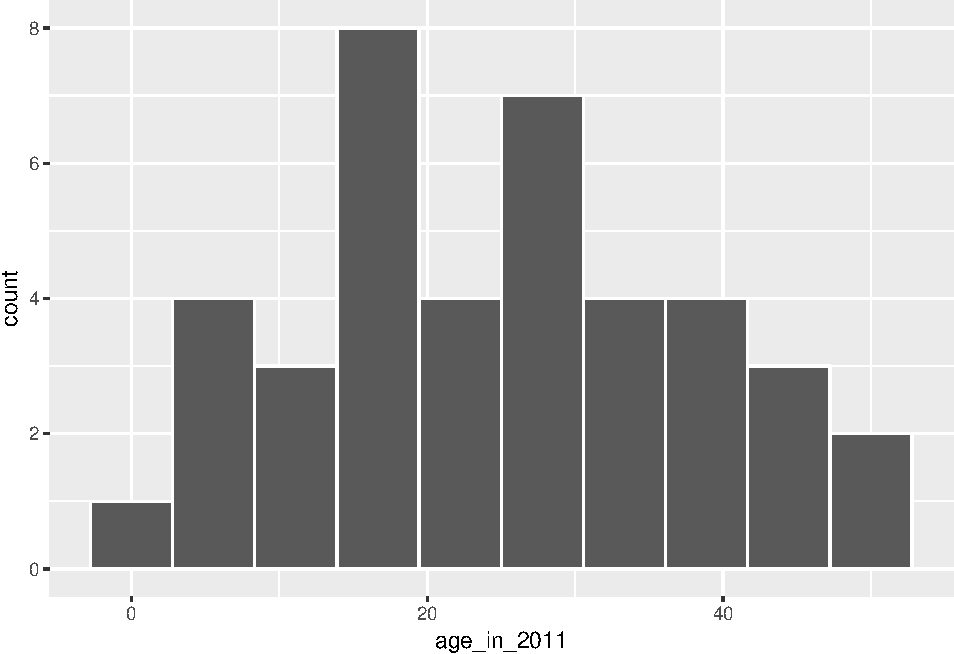
\includegraphics{DAWeek7_files/figure-latex/summary-1.pdf}

We see a roughly symmetric distribution here that has quite a few values
near 20 years in age with only a few larger than 40 years or smaller
than 5 years. If \texttt{pennies\_sample} is a representative sample
from the population, we'd expect the age of all US pennies collected in
2011 to have a similar shape, a similar spread, and similar measures of
central tendency like the mean.

So where does the mean value fall for this sample? This point will be
known as our \textbf{point estimate} and provides us with a single
number that could serve as the guess to what the true population mean
age might be. Recall how to find this using the \texttt{dplyr} package:

\begin{Shaded}
\begin{Highlighting}[]
\NormalTok{x_bar <-}\StringTok{ }\NormalTok{pennies_sample }\OperatorTok
\StringTok{  }\KeywordTok{summarize}\NormalTok{(}\DataTypeTok{stat =} \KeywordTok{mean}\NormalTok{(age_in_}\DecValTok{2011}\NormalTok{))}
\end{Highlighting}
\end{Shaded}

We've denoted this sample mean as \(\hat{x}\), which is the standard
symbol for denoting the mean of a sample. Our point estimate is, thus,
\(\hat{x}=25.1\). Note that this is just one sample providing just one
sample mean to estimate the population mean. To construct a
\textbf{confidence interval} (and to do any sort of \emph{statistical
inference} for that matter) we need to know about the \textbf{sampling
distribution} of this sample mean, i.e.~how would its values vary if
many samples of the same size were drawn from the same population.

The process of \textbf{bootstrapping} allows us to use a single sample
to generate many different samples that will act as our way of
approximating a sampling distribution using a created \textbf{bootstrap
distribution} instead. We will ``pull ourselves up by our bootstraps''
(as the saying goes in English, see here) using a single sample
(\texttt{pennies\_sample}) to get an idea of the \textbf{sampling
distribution} of the sample mean.

\subsection{The Bootstrapping Process}\label{the-bootstrapping-process}

Bootstrapping uses a process of sampling \textbf{with replacement} from
our original sample to create new \textbf{bootstrap samples} of the
\emph{same size} as our original sample. We can use the
\texttt{rep\_sample\_n()} function in the \texttt{infer} package to
explore what one such bootstrap sample would look like. Remember that we
are randomly sampling from the original sample here \textbf{with
replacement} and that we always use the same sample size for the
bootstrap samples as the size of the original sample
(\texttt{pennies\_sample}).

\begin{Shaded}
\begin{Highlighting}[]
\NormalTok{bootstrap_sample1 <-}\StringTok{ }\NormalTok{pennies_sample }\OperatorTok\StringTok{ }
\StringTok{  }\KeywordTok{rep_sample_n}\NormalTok{(}\DataTypeTok{size =} \DecValTok{40}\NormalTok{, }\DataTypeTok{replace =} \OtherTok{TRUE}\NormalTok{, }\DataTypeTok{reps =} \DecValTok{1}\NormalTok{)}

\KeywordTok{ggplot}\NormalTok{(bootstrap_sample1, }\KeywordTok{aes}\NormalTok{(}\DataTypeTok{x =}\NormalTok{ age_in_}\DecValTok{2011}\NormalTok{)) }\OperatorTok{+}
\StringTok{  }\KeywordTok{geom_histogram}\NormalTok{(}\DataTypeTok{bins =} \DecValTok{10}\NormalTok{, }\DataTypeTok{color =} \StringTok{"white"}\NormalTok{)}
\end{Highlighting}
\end{Shaded}

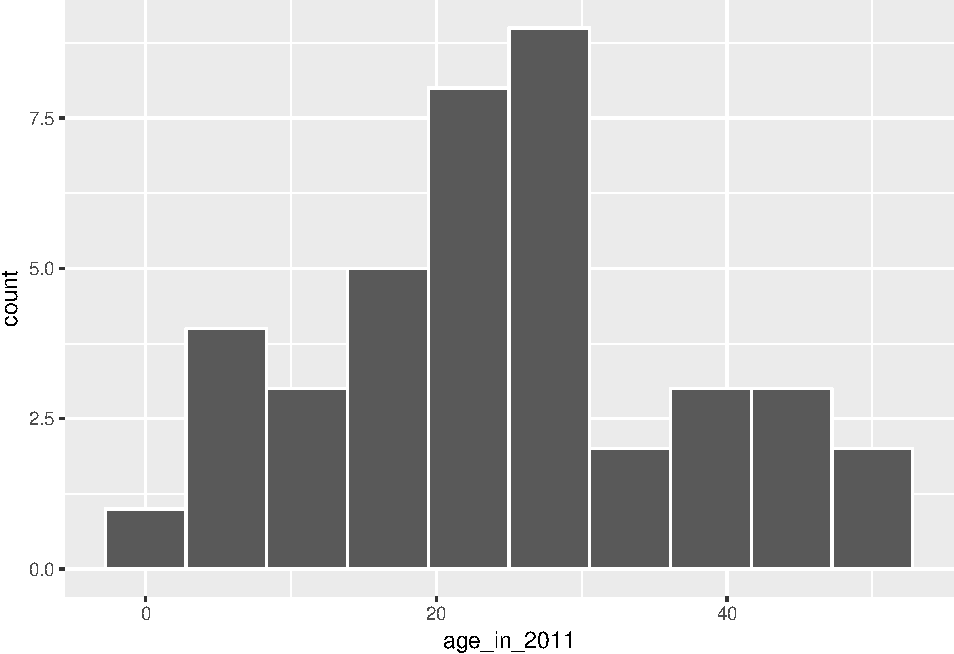
\includegraphics{DAWeek7_files/figure-latex/sample1-1.pdf}

We now have another sample from what we could assume comes from the
population of interest. We can similarly calculate the sample mean of
this bootstrap sample, called a \textbf{bootstrap statistic}.

\begin{Shaded}
\begin{Highlighting}[]
\NormalTok{bootstrap_sample1 }\OperatorTok\StringTok{ }
\StringTok{  }\KeywordTok{summarize}\NormalTok{(}\DataTypeTok{stat =} \KeywordTok{mean}\NormalTok{(age_in_}\DecValTok{2011}\NormalTok{))}
\end{Highlighting}
\end{Shaded}

\begin{verbatim}
# A tibble: 1 x 2
  replicate  stat
      <int> <dbl>
1         1  24.9
\end{verbatim}

We'll come back to analyzing the variation in the values of different
bootstrap samples' statistics shortly. But first, let's recap what was
done to get to this single bootstrap sample using a tactile explanation:

\begin{enumerate}
\def\labelenumi{\arabic{enumi}.}
\tightlist
\item
  First, pretend that each of the 40 values of \texttt{age\_in\_2011} in
  \texttt{pennies\_sample} were written on a small piece of paper.
  Recall that these values were 6, 30, 34, 19, 6, etc.
\item
  Now, put the 40 small pieces of paper into a receptacle such as a
  baseball cap.
\item
  Shake up the pieces of paper.
\item
  Draw ``at random'' from the cap to select one piece of paper.
\item
  Write down the value on this piece of paper. Say that it is 28.
\item
  Now, place this piece of paper containing 28 back into the cap.
\item
  Draw ``at random'' again from the cap to select a piece of paper. Note
  that this is the sampling with replacement part since you may draw 28
  again.
\item
  Repeat this process until you have drawn 40 pieces of paper and
  written down the values on these 40 pieces of paper. Completing this
  repetition produces ONE bootstrap sample.
\end{enumerate}

If you look at the values in \texttt{bootstrap\_sample1}, you can see
how this process plays out. We originally drew 28, then we drew 11, then
7, and so on. Of course, we didn't actually use pieces of paper and a
cap here. We just had the computer perform this process for us to
produce \texttt{bootstrap\_sample1} using \texttt{rep\_sample\_n()} with
\texttt{replace\ =\ TRUE} set.

The process of \emph{sampling with replacement} is how we can use the
original sample to take a guess as to what other values in the
population may be. Sometimes in these bootstrap samples, we will select
lots of larger values from the original sample, sometimes we will select
lots of smaller values, and most frequently we will select values that
are near the center of the sample. Let's explore what the distribution
of values of \texttt{age\_in\_2011} for six different bootstrap samples
looks like to further understand this variability.

\begin{Shaded}
\begin{Highlighting}[]
\NormalTok{six_bootstrap_samples <-}\StringTok{ }\NormalTok{pennies_sample }\OperatorTok\StringTok{ }
\StringTok{  }\KeywordTok{rep_sample_n}\NormalTok{(}\DataTypeTok{size =} \DecValTok{40}\NormalTok{, }\DataTypeTok{replace =} \OtherTok{TRUE}\NormalTok{, }\DataTypeTok{reps =} \DecValTok{6}\NormalTok{)}

\KeywordTok{ggplot}\NormalTok{(six_bootstrap_samples, }\KeywordTok{aes}\NormalTok{(}\DataTypeTok{x =}\NormalTok{ age_in_}\DecValTok{2011}\NormalTok{)) }\OperatorTok{+}
\StringTok{  }\KeywordTok{geom_histogram}\NormalTok{(}\DataTypeTok{bins =} \DecValTok{10}\NormalTok{, }\DataTypeTok{color =} \StringTok{"white"}\NormalTok{) }\OperatorTok{+}
\StringTok{  }\KeywordTok{facet_wrap}\NormalTok{(}\OperatorTok{~}\StringTok{ }\NormalTok{replicate)}
\end{Highlighting}
\end{Shaded}

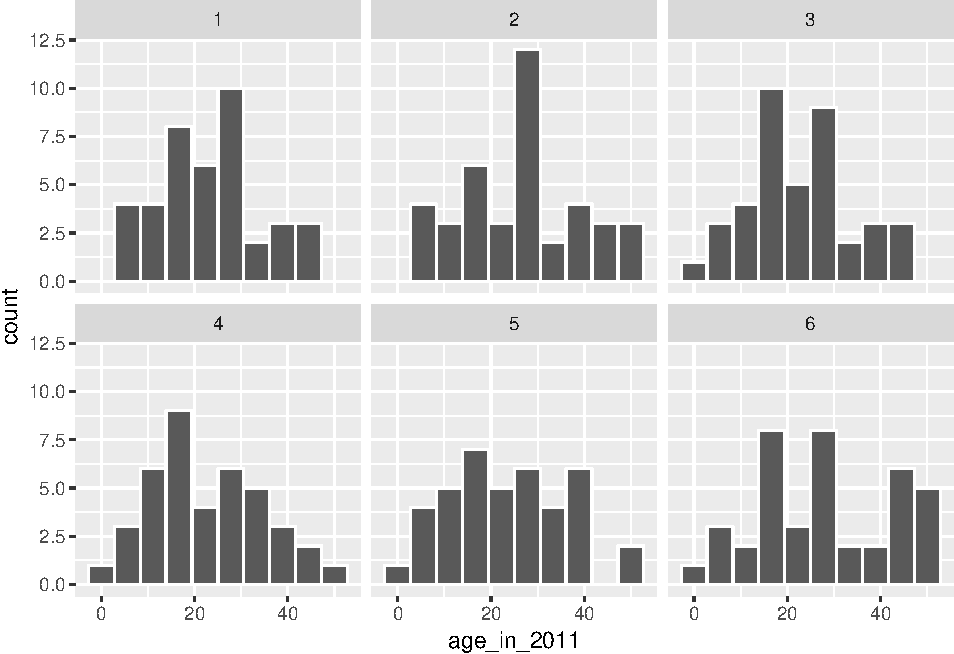
\includegraphics{DAWeek7_files/figure-latex/sample6-1.pdf}

We can also look at the six different means using \texttt{dplyr} syntax:

\begin{Shaded}
\begin{Highlighting}[]
\NormalTok{six_bootstrap_samples }\OperatorTok\StringTok{ }
\StringTok{  }\KeywordTok{group_by}\NormalTok{(replicate) }\OperatorTok\StringTok{ }
\StringTok{  }\KeywordTok{summarize}\NormalTok{(}\DataTypeTok{stat =} \KeywordTok{mean}\NormalTok{(age_in_}\DecValTok{2011}\NormalTok{))}
\end{Highlighting}
\end{Shaded}

\begin{verbatim}
# A tibble: 6 x 2
  replicate  stat
      <int> <dbl>
1         1  23.6
2         2  26.5
3         3  22.8
4         4  22.8
5         5  23.7
6         6  28.7
\end{verbatim}

Instead of doing this six times, we could do it 1000 times and then look
at the distribution of \texttt{stat} across all 1000 of the
\texttt{replicates}. This sets the stage for the \texttt{infer} R
package (see documentation here or the ``Cheat Sheet'' on the DA Moodle
page) that helps users perform statistical inference such as confidence
intervals and hypothesis tests using verbs similar to what you've seen
with \texttt{dplyr}. In the next section we'll walk through setting up
each of the infer verbs for confidence intervals using this
\texttt{pennies\_sample} example, while also explaining the purpose of
the verbs in a general framework.

\section{Infer Package for Statistical Inference}\label{sec:Infer}

The \texttt{infer} package makes great use of the \texttt{tidyverse}
``pipe'' \texttt{\%\textgreater{}\%} to create a pipeline for
statistical inference. The goal of the package is to provide a way for
its users to explain the computational process of confidence intervals
and hypothesis tests using the code as a guide. The verbs build in order
here, so you'll want to start with \texttt{specify()} and then continue
through the others as needed.

\subsection{Specify Variables}\label{specify-variables}

\begin{center}
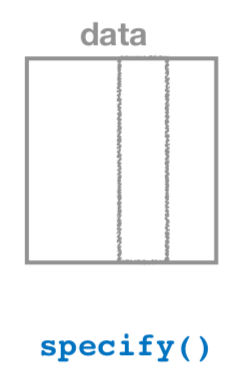
\includegraphics[width=0.25\textwidth]{specify.png}
\end{center}

The \texttt{specify()} function is used primarily to choose which
variables will be the focus of the statistical inference. In addition, a
setting of which variable will act as the \texttt{explanatory} and which
acts as the \texttt{response} variable is done here. For proportion
problems (i.e.~Scenarios 1 \& 3 in Table 1) we also specify which of the
different levels we are calculating the proportion of (e.g. ``females'',
``approve of Obama's job performance'', etc.). To begin to create a
confidence interval for the population mean age of US pennies in 2011,
we start by using \texttt{specify()} to choose which variable in our
\texttt{pennies\_sample} data we'd like to work with. This can be done
in one of two ways:

\begin{enumerate}
\def\labelenumi{\arabic{enumi}.}
\tightlist
\item
  Using the \texttt{response} argument:
\end{enumerate}

\begin{Shaded}
\begin{Highlighting}[]
\NormalTok{pennies_sample }\OperatorTok\StringTok{ }
\StringTok{  }\KeywordTok{specify}\NormalTok{(}\DataTypeTok{response =}\NormalTok{ age_in_}\DecValTok{2011}\NormalTok{)}
\end{Highlighting}
\end{Shaded}

\begin{verbatim}
Response: age_in_2011 (integer)
# A tibble: 40 x 1
   age_in_2011
         <int>
 1           6
 2          30
 3          34
 4          19
 5           6
 6           5
 7          11
 8          19
 9          23
10          15
# ... with 30 more rows
\end{verbatim}

\begin{enumerate}
\def\labelenumi{\arabic{enumi}.}
\setcounter{enumi}{1}
\tightlist
\item
  Using \texttt{formula} notation:
\end{enumerate}

\begin{Shaded}
\begin{Highlighting}[]
\NormalTok{pennies_sample }\OperatorTok\StringTok{ }
\StringTok{  }\KeywordTok{specify}\NormalTok{(}\DataTypeTok{formula =}\NormalTok{ age_in_}\DecValTok{2011} \OperatorTok{~}\StringTok{ }\OtherTok{NULL}\NormalTok{)}
\end{Highlighting}
\end{Shaded}

\begin{verbatim}
Response: age_in_2011 (integer)
# A tibble: 40 x 1
   age_in_2011
         <int>
 1           6
 2          30
 3          34
 4          19
 5           6
 6           5
 7          11
 8          19
 9          23
10          15
# ... with 30 more rows
\end{verbatim}

Note that the formula notation uses the common R methodology to include
the response \(y\) variable on the left of the
\texttt{\textasciitilde{}} and the explanatory \(x\) variable on the
right of the ``tilde.'' Recall that you used this notation frequently
with the \texttt{lm()} function in Weeks 4 and 6 when fitting regression
models. Either notation works just fine, but a preference is usually
given here for the \texttt{formula} notation to further build on the
ideas from earlier chapters.

\subsection{Generate Replicates}\label{generate-replicates}

\begin{center}
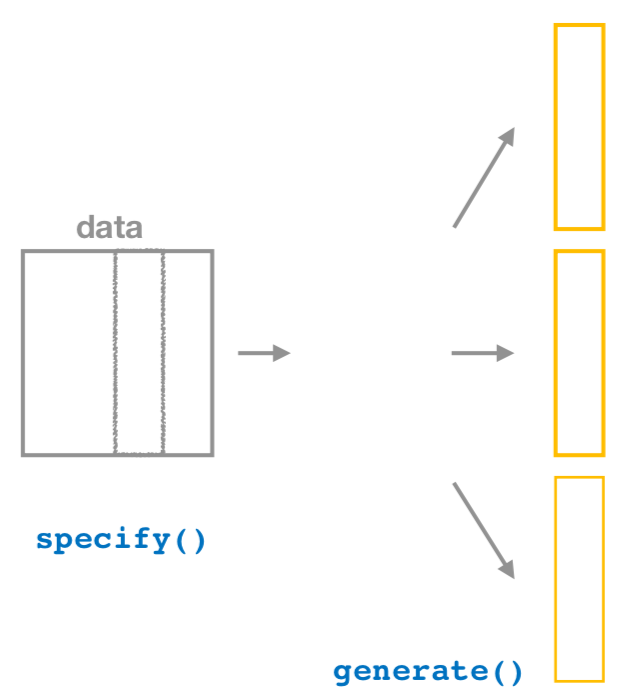
\includegraphics[width=0.5\textwidth]{generate.png}
\end{center}

After \texttt{specify()ing} the variables we'd like in our inferential
analysis, we next feed that into the \texttt{generate()} verb. The
\texttt{generate()} verb's main argument is \texttt{reps}, which is used
to give how many different repetitions one would like to perform.
Another argument here is \texttt{type}, which is automatically
determined by the kinds of variables passed into \texttt{specify()}. We
can also be explicit and set this \texttt{type} to be
\texttt{type\ =\ "bootstrap"}. Make sure to check out \texttt{?generate}
to see the options here and use the \texttt{?} operator to better
understand other verbs as well. Let's \texttt{generate()} 1000 bootstrap
samples:

\begin{Shaded}
\begin{Highlighting}[]
\NormalTok{thousand_bootstrap_samples <-}\StringTok{ }\NormalTok{pennies_sample }\OperatorTok
\StringTok{  }\KeywordTok{specify}\NormalTok{(}\DataTypeTok{response =}\NormalTok{ age_in_}\DecValTok{2011}\NormalTok{) }\OperatorTok
\StringTok{  }\KeywordTok{generate}\NormalTok{(}\DataTypeTok{reps =} \DecValTok{1000}\NormalTok{, }\DataTypeTok{type =} \StringTok{"bootstrap"}\NormalTok{)}
\end{Highlighting}
\end{Shaded}

We can use the \texttt{dplyr} \texttt{count()} function to help us
understand what the \texttt{thousand\_bootstrap\_samples} data frame
looks like:

\begin{Shaded}
\begin{Highlighting}[]
\NormalTok{thousand_bootstrap_samples }\OperatorTok\StringTok{ }\KeywordTok{count}\NormalTok{(replicate)}
\end{Highlighting}
\end{Shaded}

\begin{verbatim}
# A tibble: 1,000 x 2
# Groups:   replicate [1,000]
   replicate     n
       <int> <int>
 1         1    40
 2         2    40
 3         3    40
 4         4    40
 5         5    40
 6         6    40
 7         7    40
 8         8    40
 9         9    40
10        10    40
# ... with 990 more rows
\end{verbatim}

\begin{Shaded}
\begin{Highlighting}[]
\CommentTok{# Equivalent to:}
\CommentTok{# thousand_bootstrap_samples %>% }
\CommentTok{#   group_by(replicate) %>% }
\CommentTok{#   summarise(n=n())}
\end{Highlighting}
\end{Shaded}

Notice that each \texttt{replicate} has 40 entries here. Now that we
have 1000 different bootstrap samples, our next step is to
\texttt{calculate} the bootstrap statistics for each sample.

\subsection{Calculate Summary
Statistics}\label{calculate-summary-statistics}

\begin{center}
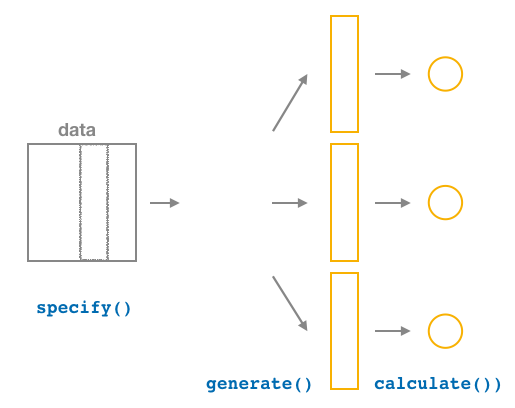
\includegraphics[width=0.5\textwidth]{calculate.png}
\end{center}

After \texttt{generate()}ing many different samples, we next want to
condense those samples down into a single statistic for each
\texttt{replicate}d sample. As seen in the diagram, the
\texttt{calculate()} function is helpful here.

As we did at the beginning of this chapter, we now want to calculate the
mean \texttt{age\_in\_2011} for each bootstrap sample. To do so, we use
the \texttt{stat} argument and set it to \texttt{"mean"} below. The
\texttt{stat} argument has a variety of different options here and we
will see further examples of this throughout the remaining chapters.

\begin{Shaded}
\begin{Highlighting}[]
\NormalTok{bootstrap_distribution <-}\StringTok{ }\NormalTok{pennies_sample }\OperatorTok\StringTok{ }
\StringTok{  }\KeywordTok{specify}\NormalTok{(}\DataTypeTok{response =}\NormalTok{ age_in_}\DecValTok{2011}\NormalTok{) }\OperatorTok\StringTok{ }
\StringTok{  }\KeywordTok{generate}\NormalTok{(}\DataTypeTok{reps =} \DecValTok{1000}\NormalTok{) }\OperatorTok\StringTok{ }
\StringTok{  }\KeywordTok{calculate}\NormalTok{(}\DataTypeTok{stat =} \StringTok{"mean"}\NormalTok{)}
\NormalTok{bootstrap_distribution}
\end{Highlighting}
\end{Shaded}

\begin{verbatim}
# A tibble: 1,000 x 2
   replicate  stat
       <int> <dbl>
 1         1  25.9
 2         2  24.7
 3         3  20.4
 4         4  24.3
 5         5  24.7
 6         6  28.0
 7         7  24.8
 8         8  25.6
 9         9  26.6
10        10  25.0
# ... with 990 more rows
\end{verbatim}

\textbf{Observed statistic / point estimate calculations} Just as
\texttt{group\_by()\ \%\textgreater{}\%\ summarize()} produces a useful
workflow in \texttt{dplyr}, we can also use
\texttt{specify()\ \%\textgreater{}\%\ calculate()} to compute summary
measures on our original sample data. It's often helpful both in
confidence interval calculations and in hypothesis testing to identify
what the corresponding statistic is in the original data. For our
example on penny age, we computed above a value of \texttt{x\_bar} using
the \texttt{summarize()} verb in \texttt{dplyr}:

\begin{Shaded}
\begin{Highlighting}[]
\NormalTok{pennies_sample }\OperatorTok\StringTok{ }
\StringTok{  }\KeywordTok{summarize}\NormalTok{(}\DataTypeTok{stat =} \KeywordTok{mean}\NormalTok{(age_in_}\DecValTok{2011}\NormalTok{))}
\end{Highlighting}
\end{Shaded}

\begin{verbatim}
# A tibble: 1 x 1
   stat
  <dbl>
1  25.1
\end{verbatim}

This can also be done by skipping the \texttt{generate()} step in the
pipeline feeding \texttt{specify()} directly into \texttt{calculate()}:

\begin{Shaded}
\begin{Highlighting}[]
\NormalTok{pennies_sample }\OperatorTok\StringTok{ }
\StringTok{  }\KeywordTok{specify}\NormalTok{(}\DataTypeTok{response =}\NormalTok{ age_in_}\DecValTok{2011}\NormalTok{) }\OperatorTok\StringTok{ }
\StringTok{  }\KeywordTok{calculate}\NormalTok{(}\DataTypeTok{stat =} \StringTok{"mean"}\NormalTok{)}
\end{Highlighting}
\end{Shaded}

\begin{verbatim}
# A tibble: 1 x 1
   stat
  <dbl>
1  25.1
\end{verbatim}

This shortcut will be particularly useful when the calculation of the
observed statistic is tricky to do using \texttt{dplyr} alone. This is
particularly the case when working with more than one variable.

\subsection{Visualize the Results}\label{visualize-the-results}

\begin{center}
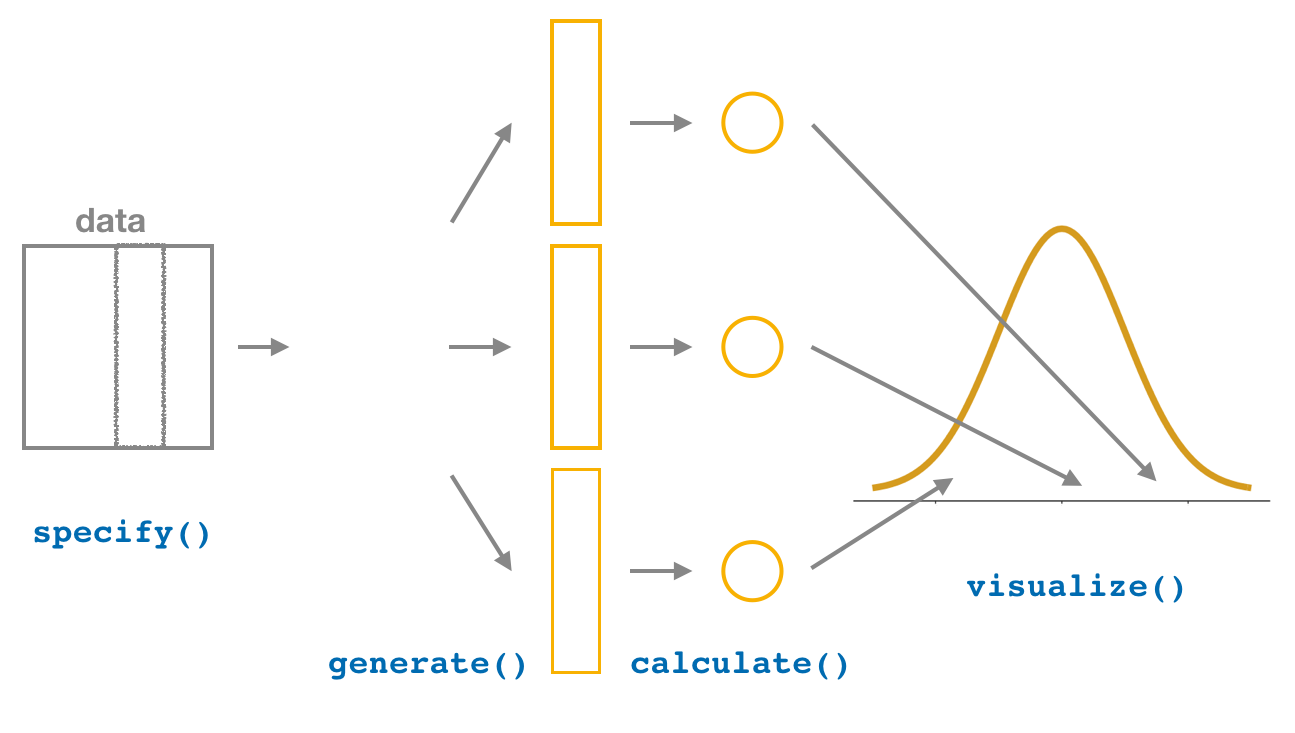
\includegraphics[width=0.5\textwidth]{visualize.png}
\end{center}

The \texttt{visualize()} verb provides a simple way to view the
bootstrap distribution as a histogram of the \texttt{stat} variable
values. It has many other arguments that one can use as well including
the shading of the histogram values corresponding to the confidence
interval values.

\begin{Shaded}
\begin{Highlighting}[]
\NormalTok{bootstrap_distribution }\OperatorTok
\StringTok{  }\KeywordTok{visualize}\NormalTok{()}
\end{Highlighting}
\end{Shaded}

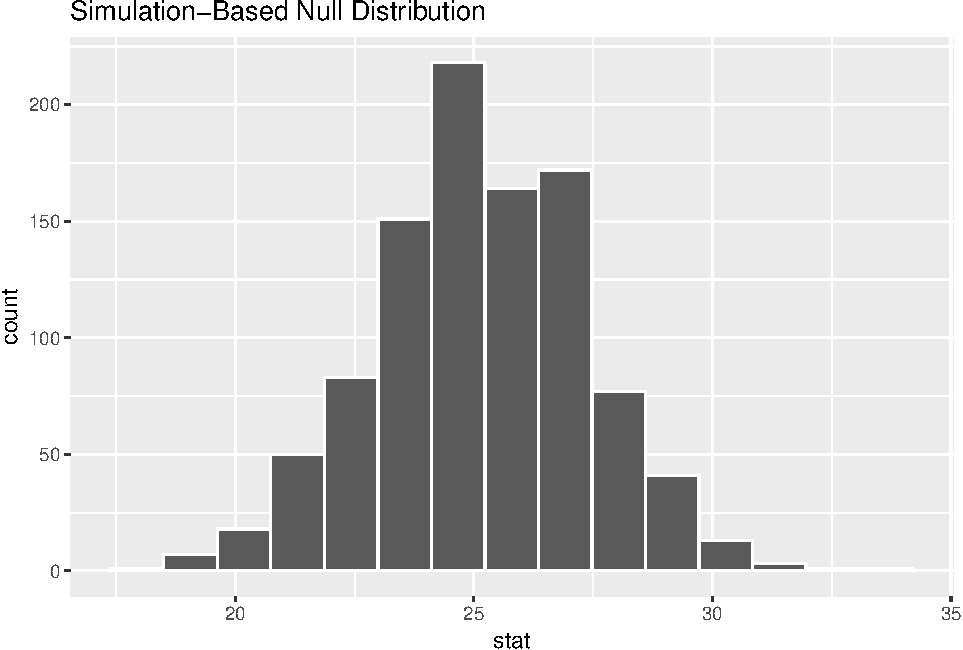
\includegraphics{DAWeek7_files/figure-latex/visualize-1.pdf}

The shape of this resulting distribution may look familiar to you. It
resembles the well-known normal (bell-shaped) curve. It is, in fact, an
estimate of the \textbf{sampling variability} of the sample statistic.
If you think back to \emph{Statistical Inference} in Semester 1 you will
remember that the \emph{Central Limit Theorem} predicted that the
sampling distribution would be a \textbf{normal distribution}, as seen
in the bell-shaped distribution here.

The following diagram recaps the \texttt{infer} pipeline for creating a
bootstrap distribution.

\begin{center}
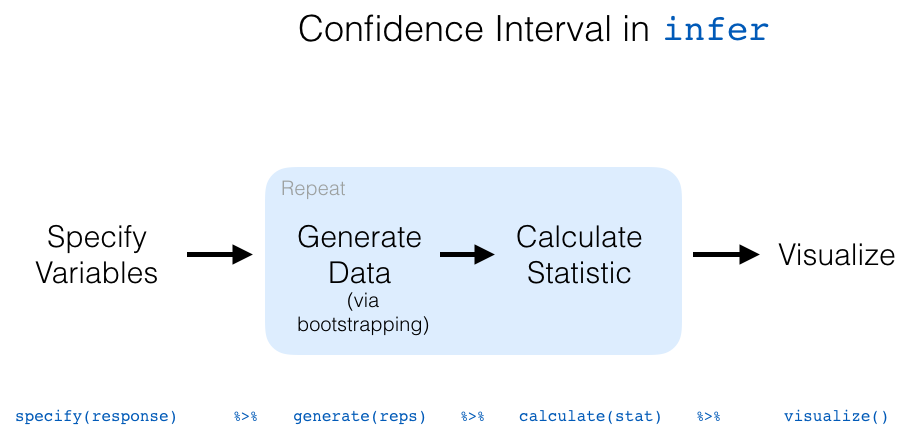
\includegraphics[width=0.5\textwidth]{ci_diagram.png}
\end{center}

\section{Constructing Confidence Intervals}\label{sec:CI}

\textbf{confidence interval}: a range of plausible values for a
population parameter. It depends on a specified confidence level with
higher \emph{confidence levels} corresponding to wider confidence
intervals and lower confidence levels corresponding to narrower
confidence intervals. Common confidence levels include 90\%, 95\%, and
99\%.

\textbf{Confidence intervals} play an important role in the sciences and
any field that uses data. You can think of a confidence interval as
playing the role of a net when fishing. Instead of just trying to catch
a fish with a single spear (estimating an unknown parameter by using a
single point estimate/sample statistic), we can use a net to try to
provide a range of possible locations for the fish (use a range of
possible values based around our sample statistic to make a plausible
guess as to the location of the parameter).

The bootstrapping process provides bootstrap statistics that have a
bootstrap distribution with center at (or extremely close to) the mean
of the original sample. This can be seen by giving the observed
statistic \texttt{obs\_stat} argument the value of the point estimate
\texttt{x\_bar}.

\begin{Shaded}
\begin{Highlighting}[]
\NormalTok{bootstrap_distribution }\OperatorTok
\StringTok{  }\KeywordTok{visualize}\NormalTok{(}\DataTypeTok{obs_stat =}\NormalTok{ x_bar)}
\end{Highlighting}
\end{Shaded}

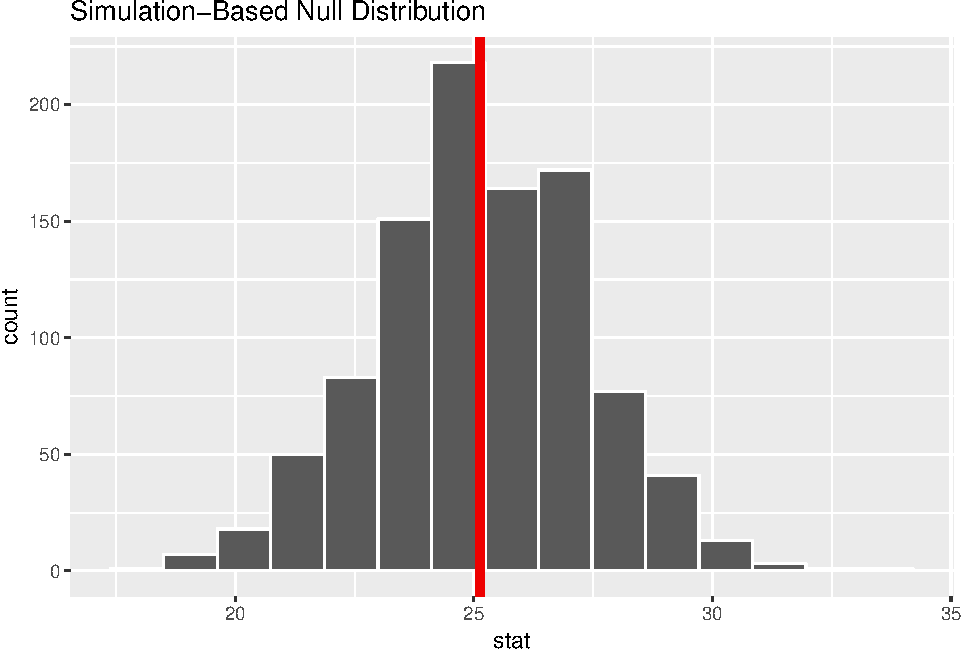
\includegraphics{DAWeek7_files/figure-latex/visualize2-1.pdf}

We can also compute the mean of the bootstrap distribution of means to
see how it compares to \texttt{x\_bar}:

\begin{Shaded}
\begin{Highlighting}[]
\NormalTok{bootstrap_distribution }\OperatorTok
\StringTok{  }\KeywordTok{summarize}\NormalTok{(}\DataTypeTok{mean_of_means =} \KeywordTok{mean}\NormalTok{(stat))}
\end{Highlighting}
\end{Shaded}

\begin{verbatim}
# A tibble: 1 x 1
  mean_of_means
          <dbl>
1          25.1
\end{verbatim}

\subsection{The Percentile Method}\label{the-percentile-method}

One way to calculate a range of plausible values for the unknown mean
age of coins in 2011 is to use the middle 95\% of the
\texttt{bootstrap\_distribution} to determine our endpoints. Our
endpoints are thus at the 2.5th and 97.5th percentiles. This can be done
with \texttt{infer} using the \texttt{get\_ci()} function. (You can also
use the \texttt{conf\_int()} or \texttt{get\_confidence\_interval()}
functions here as they are aliases that work the exact same way.)

\begin{Shaded}
\begin{Highlighting}[]
\NormalTok{bootstrap_distribution }\OperatorTok\StringTok{ }
\StringTok{  }\KeywordTok{get_ci}\NormalTok{(}\DataTypeTok{level =} \FloatTok{0.95}\NormalTok{, }\DataTypeTok{type =} \StringTok{"percentile"}\NormalTok{)}
\end{Highlighting}
\end{Shaded}

\begin{verbatim}
# A tibble: 1 x 2
  `2.5%` `97.5%`
   <dbl>   <dbl>
1   20.6    29.4
\end{verbatim}

These options are the default values for \texttt{level} and
\texttt{type} so we can also just do:

\begin{Shaded}
\begin{Highlighting}[]
\NormalTok{percentile_ci <-}\StringTok{ }\NormalTok{bootstrap_distribution }\OperatorTok\StringTok{ }
\StringTok{  }\KeywordTok{get_ci}\NormalTok{()}
\NormalTok{percentile_ci}
\end{Highlighting}
\end{Shaded}

\begin{verbatim}
# A tibble: 1 x 2
  `2.5%` `97.5%`
   <dbl>   <dbl>
1   20.6    29.4
\end{verbatim}

Using the percentile method, our range of plausible values for the mean
age of US pennies in circulation in 2011 is 20.97 years to 29.25 years.
We can use the \texttt{visualize()} function to view this using the
\texttt{endpoints} and \texttt{direction} arguments, setting
\texttt{direction} to \texttt{"between"} (between the values) and
\texttt{endpoints} to be those stored with name \texttt{percentile\_ci}.

\begin{Shaded}
\begin{Highlighting}[]
\NormalTok{bootstrap_distribution }\OperatorTok\StringTok{ }
\StringTok{  }\KeywordTok{visualize}\NormalTok{(}\DataTypeTok{endpoints =}\NormalTok{ percentile_ci, }\DataTypeTok{direction =} \StringTok{"between"}\NormalTok{)}
\end{Highlighting}
\end{Shaded}

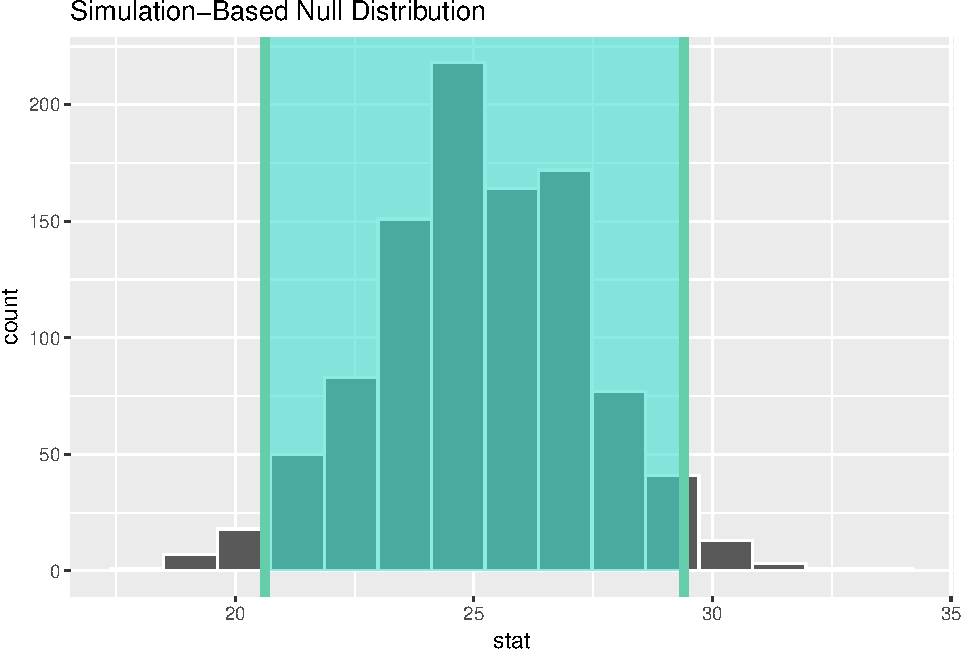
\includegraphics{DAWeek7_files/figure-latex/visualize3-1.pdf}

You can see that 95\% of the data stored in the \texttt{stat} variable
in \texttt{bootstrap\_distribution} falls between the two endpoints with
2.5\% to the left outside of the shading and 2.5\% to the right outside
of the shading. The cut-off points that provide our range are shown with
the darker lines.

\subsection{The Standard Error Method}\label{the-standard-error-method}

If the bootstrap distribution is close to symmetric and bell-shaped, we
can also use a shortcut formula for determining the lower and upper
endpoints of the confidence interval. This is done by using the formula
\(\bar{x}?(multiplier???SE)\), where \(\bar{x}\) is our original sample
mean and \(SE\) stands for \textbf{standard error} and corresponds to
the standard deviation of the bootstrap distribution.

\textbf{Definition}: The \emph{standard error} is the standard deviation
of the sampling distribution.

The variability of the sampling distribution may be approximated by the
variability of the bootstrap distribution. Traditional theory-based
methodologies for inference also have formulas for standard errors,
assuming some conditions are met (you will have (seen some of
these){[}\url{https://moodle.gla.ac.uk/pluginfile.php/1813455/mod_resource/content/1/Interval\%20Estimates\%20Summary.pdf}{]}
in Statistical Inference in Semester 1).

The value of \emph{multiplier} here is the appropriate percentile of the
standard normal distribution. This is automatically calculated when
\texttt{level} is provided with \texttt{level\ =\ 0.95} being the
default. (95\% of the values in a standard normal distribution fall
within 1.96 standard deviations of the mean, so
\texttt{multiplier\ =\ 1.96} corresponds to \texttt{level\ =\ 0.95}, for
example.) As mentioned, this formula assumes that the bootstrap
distribution is symmetric and bell-shaped. This is often the case with
bootstrap distributions, especially those in which the original
distribution of the sample is not highly skewed.

This \(\bar{x}?(multiplier???SE)\) formula is implemented in the
\texttt{get\_ci()} function as shown with our pennies problem using the
bootstrap distribution's variability as an approximation for the
sampling distribution's variability. We'll see more on this
approximation shortly.

Note that the center of the confidence interval (the
\texttt{point\_estimate}) must be provided for the standard error
confidence interval.

\begin{Shaded}
\begin{Highlighting}[]
\NormalTok{standard_error_ci <-}\StringTok{ }\NormalTok{bootstrap_distribution }\OperatorTok\StringTok{ }
\StringTok{  }\KeywordTok{get_ci}\NormalTok{(}\DataTypeTok{type =} \StringTok{"se"}\NormalTok{, }\DataTypeTok{point_estimate =}\NormalTok{ x_bar)}
\NormalTok{standard_error_ci}
\end{Highlighting}
\end{Shaded}

\begin{verbatim}
# A tibble: 1 x 2
  lower upper
  <dbl> <dbl>
1  20.8  29.5
\end{verbatim}

\begin{Shaded}
\begin{Highlighting}[]
\NormalTok{bootstrap_distribution }\OperatorTok\StringTok{ }
\StringTok{  }\KeywordTok{visualize}\NormalTok{(}\DataTypeTok{endpoints =}\NormalTok{ standard_error_ci, }\DataTypeTok{direction =} \StringTok{"between"}\NormalTok{)}
\end{Highlighting}
\end{Shaded}

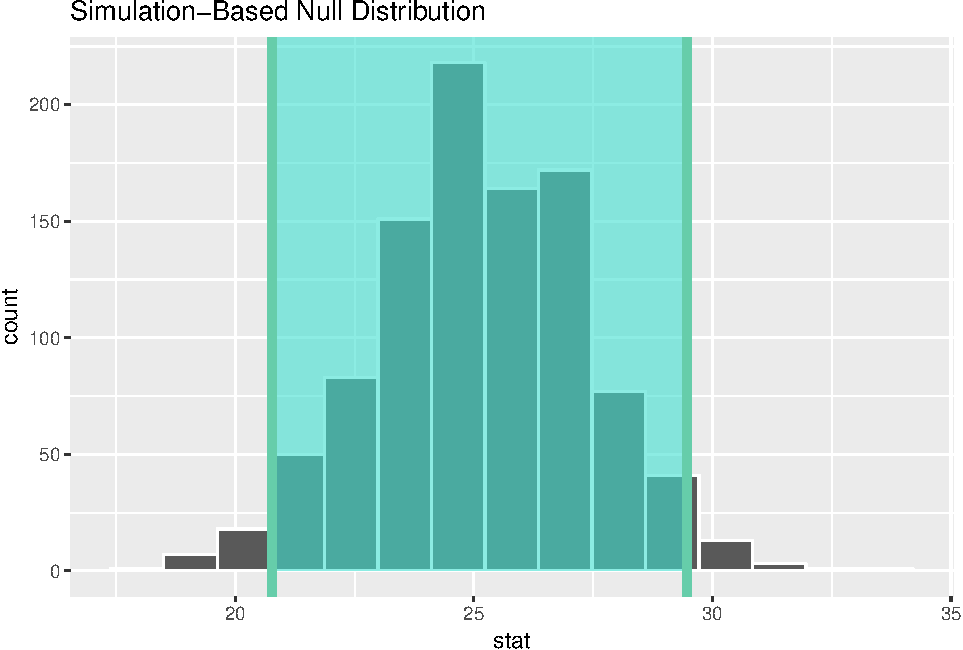
\includegraphics{DAWeek7_files/figure-latex/get_ci3-1.pdf}

We see that both methods produce nearly identical confidence intervals
with the percentile method being {[}\(20.97,29.25\){]} and the standard
error method being {[}\(20.97,29.28\){]}.

\section{Interpreting the Confidence
Interval}\label{interpreting-the-confidence-interval}

Recall that the confidence intervals we've produced are based on
bootstrapping using the single sample \texttt{pennies\_sample}. We have
been claiming that this is a sample from all the pennies in circulation
in 2011, but we can now reveal that it is actually a sample from a
larger number of pennies stored as \texttt{pennies} in the
\texttt{moderndive} package. The \texttt{pennies} data frame contains
800 rows of data and two columns pertaining to the same variables as
\texttt{pennies\_sample}. Its important to stress that this is
\emph{very artificial}, i.e.~we would usually never have access to all
the information about the larger group from which our sample is taken,
but we have set up the data this way here to illustrate the properties
of confidence intervals for the purpose of interpreting confidence
intervals.

So let's assume that \texttt{pennies} is our population of interest
(i.e.~a population with \(N=800\) units). We can therefor calculate the
population mean age of pennies in 2011, denoted by the Greek letter
\(\mu\), by calculating the mean of \texttt{age\_in\_2011} for the
\texttt{pennies} data frame.

\begin{Shaded}
\begin{Highlighting}[]
\NormalTok{pennies_mu <-}\StringTok{ }\NormalTok{pennies }\OperatorTok\StringTok{ }
\StringTok{  }\KeywordTok{summarize}\NormalTok{(}\DataTypeTok{overall_mean =} \KeywordTok{mean}\NormalTok{(age_in_}\DecValTok{2011}\NormalTok{)) }\OperatorTok\StringTok{ }
\StringTok{  }\KeywordTok{pull}\NormalTok{()  }\CommentTok{#Use this function to extract the single value from the data frame}
\NormalTok{pennies_mu}
\end{Highlighting}
\end{Shaded}

\begin{verbatim}
[1] 21.1525
\end{verbatim}

As we saw at the end of the previous section, one range of plausible
values for the population mean age of pennies in 2011 (\(\mu\)), is
{[}\(20.97,29.25\){]}. Note that the value \(\mu=21.15\) (i.e.the mean
of \texttt{pennies} calculated above) \textbf{does} fall in this
confidence interval. So in this instance, the confidence interval based
on \texttt{pennies\_sample} was a good estimate of \(\mu\).

If we had a different sample of size 40 and constructed a confidence
interval using the same method, would we be guaranteed that it contained
the population parameter value \(\mu\) as well? Let's try it out:

\begin{Shaded}
\begin{Highlighting}[]
\NormalTok{pennies_sample2 <-}\StringTok{ }\NormalTok{pennies }\OperatorTok
\StringTok{  }\KeywordTok{sample_n}\NormalTok{(}\DataTypeTok{size =} \DecValTok{40}\NormalTok{)}
\end{Highlighting}
\end{Shaded}

Note the use of the \texttt{sample\_n()} function in the \texttt{dplyr}
package here. This does the same thing as
\texttt{rep\_sample\_n(reps\ =\ 1)} but omits the extra replicate
column.

We next create an \texttt{infer} pipeline to generate a percentile-based
95\% confidence interval for \(\mu\):

\begin{Shaded}
\begin{Highlighting}[]
\NormalTok{percentile_ci2 <-}\StringTok{ }\NormalTok{pennies_sample2 }\OperatorTok\StringTok{ }
\StringTok{  }\KeywordTok{specify}\NormalTok{(}\DataTypeTok{formula =}\NormalTok{ age_in_}\DecValTok{2011} \OperatorTok{~}\StringTok{ }\OtherTok{NULL}\NormalTok{) }\OperatorTok\StringTok{ }
\StringTok{  }\KeywordTok{generate}\NormalTok{(}\DataTypeTok{reps =} \DecValTok{1000}\NormalTok{) }\OperatorTok\StringTok{ }
\StringTok{  }\KeywordTok{calculate}\NormalTok{(}\DataTypeTok{stat =} \StringTok{"mean"}\NormalTok{) }\OperatorTok\StringTok{ }
\StringTok{  }\KeywordTok{get_ci}\NormalTok{()}
\NormalTok{percentile_ci2}
\end{Highlighting}
\end{Shaded}

\begin{verbatim}
# A tibble: 1 x 2
  `2.5%` `97.5%`
   <dbl>   <dbl>
1   17.8    25.1
\end{verbatim}

This new confidence interval also contains the value of \(\mu\). Let's
further investigate by repeating this process 100 times to get 100
different confidence intervals derived from 100 different samples of
\texttt{pennies}. Each sample will have size of 40 just as the original
sample. We will plot each of these confidence intervals as horizontal
lines. We will also show a line corresponding to the known population
value of 21.1525 years.

\begin{center}
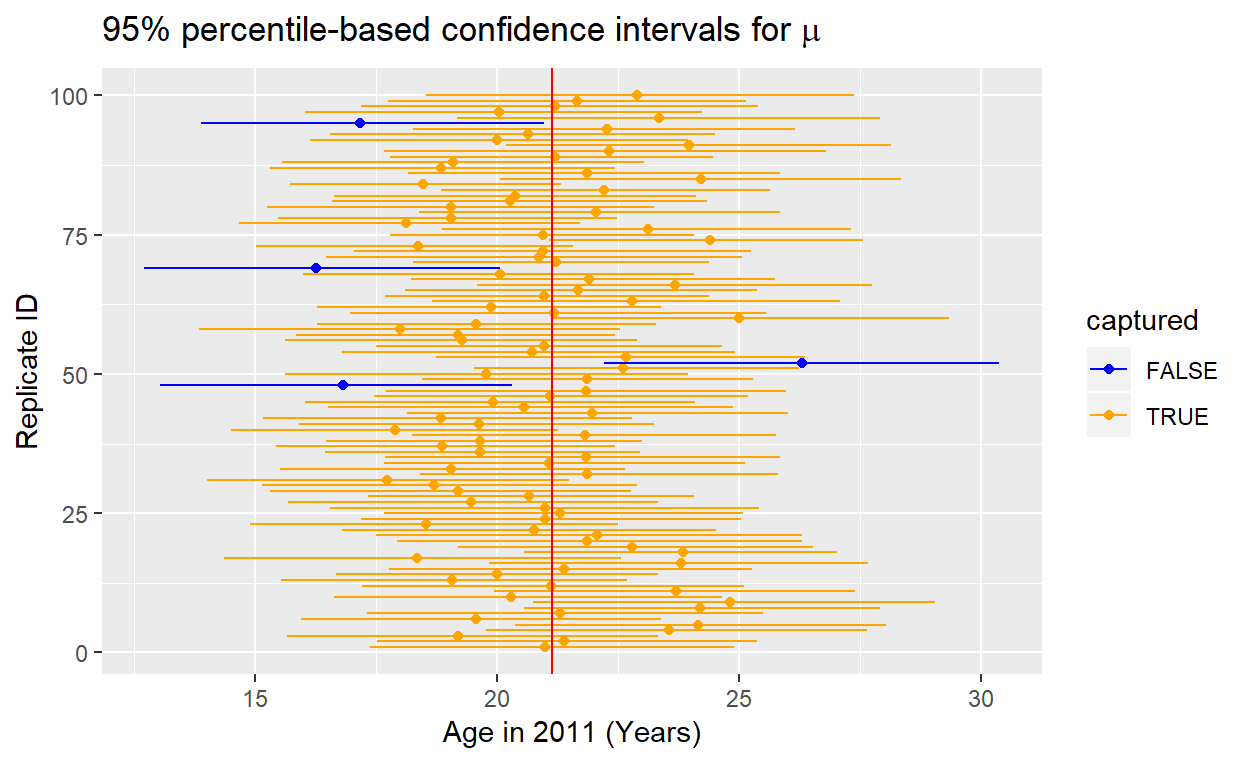
\includegraphics[width=0.5\textwidth]{ci_95.png}
\end{center}

Of the 100 confidence intervals based on samples of size \(n = 40\), 96
of them captured the population mean \(\mu=21.15\), whereas 4 of them
did not include it. If we repeated this process of building confidence
intervals more times with more samples, we'd expect 95\% of them to
contain the population mean. In other words, the procedure we have used
to generate confidence intervals is ``95\% reliable'' in that we can
expect it to include the true population parameter 95\% of the time if
the process is repeated.

To further accentuate this point, let's perform a similar procedure
using 90\% confidence intervals instead. This time we will use the
standard error method instead of the percentile method for computing the
confidence intervals.

\begin{center}
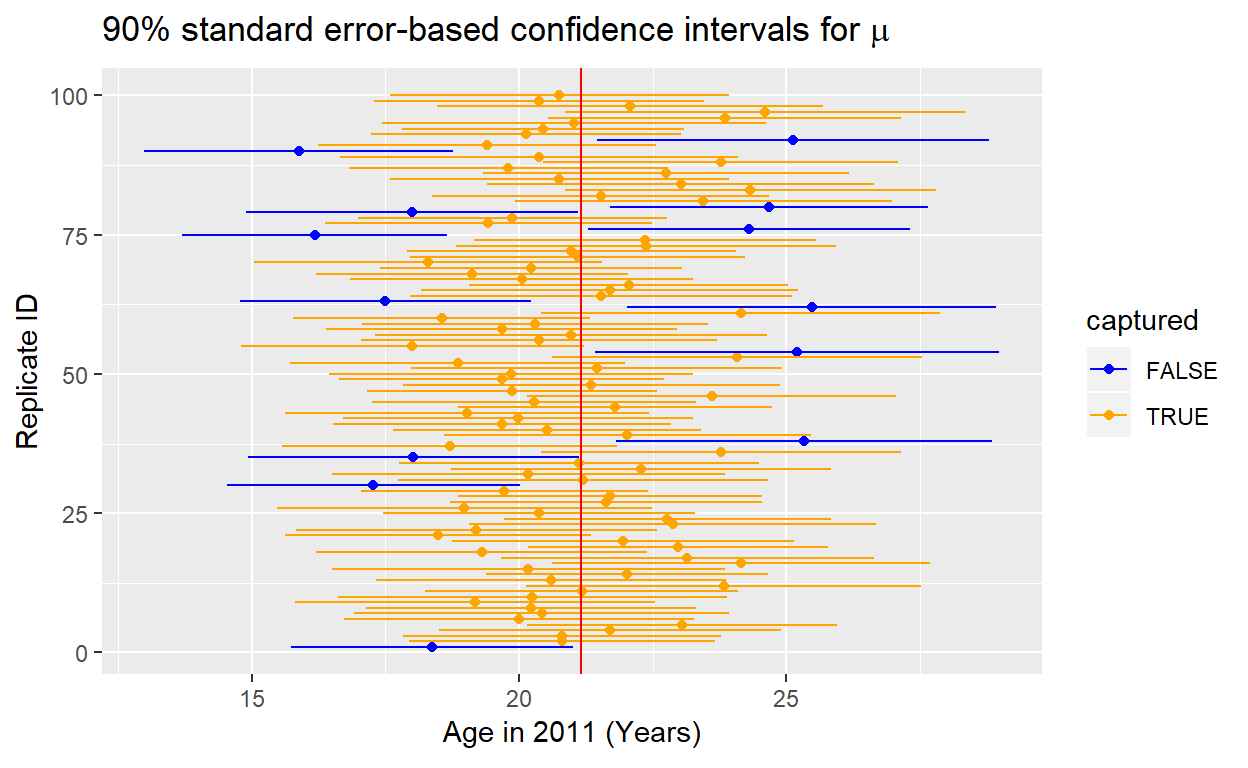
\includegraphics[width=0.5\textwidth]{ci_90.png}
\end{center}

Repeating this process for more samples would result in us getting
closer and closer to 90\% of the confidence intervals including the true
value. It is common to say while interpreting a confidence interval to
be ``95\% confident'' or ``90\% confident'' that the specified
confidence interval contains the true value. We will use this
``confident'' language throughout the rest of this chapter, but remember
that it is a theoretical statement about what we would expect to happen
if we to sample again and again from the same population (which we don't
do in practice, of course).

\section{Comparing Two Proportions}\label{comparing-two-proportions}

Let's start with an example. If you see someone else yawn, are you more
likely to yawn? In an episode of the TV show Mythbusters, they tested
the myth that yawning is contagious. Fifty adults who thought they were
being considered for an appearance on the show were interviewed by a
show recruiter (``confederate'') who either yawned or did not.
Participants then sat by themselves in a large van and were asked to
wait. While in the van, the Mythbusters watched via hidden camera to see
if the unaware participants yawned. The data frame containing the
results is available at \texttt{mythbusters\_yawn} in the
\texttt{moderndive} package. Let's check it out.

\begin{Shaded}
\begin{Highlighting}[]
\NormalTok{mythbusters_yawn}
\end{Highlighting}
\end{Shaded}

\begin{verbatim}
# A tibble: 50 x 3
    subj group   yawn 
   <int> <chr>   <chr>
 1     1 seed    yes  
 2     2 control yes  
 3     3 seed    no   
 4     4 seed    yes  
 5     5 seed    no   
 6     6 control no   
 7     7 seed    yes  
 8     8 control no   
 9     9 control no   
10    10 seed    no   
# ... with 40 more rows
\end{verbatim}

\begin{itemize}
\tightlist
\item
  The participant ID is stored in the \texttt{subj} variable with values
  of 1 to 50.
\item
  The \texttt{group} variable is either \texttt{"seed"} for when a
  confederate was trying to influence the participant or
  \texttt{"control"} if a confederate did not interact with the
  participant.
\item
  The \texttt{yawn} variable is either \texttt{"yes"} if the participant
  yawned or \texttt{"no"} if the participant did not yawn.
\end{itemize}

We can use the \texttt{janitor} package to get a glimpse into this data
in a table format:

\begin{Shaded}
\begin{Highlighting}[]
\NormalTok{mythbusters_yawn }\OperatorTok
\StringTok{  }\KeywordTok{tabyl}\NormalTok{(group, yawn) }\OperatorTok
\StringTok{  }\KeywordTok{adorn_percentages}\NormalTok{() }\OperatorTok
\StringTok{  }\KeywordTok{adorn_pct_formatting}\NormalTok{() }\OperatorTok
\StringTok{  }\KeywordTok{adorn_ns}\NormalTok{() }\CommentTok{# To show original counts}
\end{Highlighting}
\end{Shaded}

\begin{verbatim}
   group         no        yes
 control 75.0% (12) 25.0%  (4)
    seed 70.6% (24) 29.4% (10)
\end{verbatim}

We are interested in comparing the proportion of those that yawned after
seeing a \texttt{seed} versus those that yawned with no seed interaction
(i.e. \texttt{control}). We'd like to see if the difference between
these two proportions is significantly larger than 0. If so, we'd have
evidence to support the claim that yawning is contagious based on this
study.

In looking over this problem, we can take note of some important details
to include in our \texttt{infer} pipeline:

\begin{itemize}
\tightlist
\item
  We are calling a ``\texttt{success}'' having a \texttt{yawn} value of
  \texttt{yes}.
\item
  Our response variable will always correspond to the variable used in
  the \texttt{success} so the response variable is \texttt{yawn}.
\item
  The explanatory variable is the other variable of interest here:
  \texttt{group}.
\end{itemize}

\subsection{Compute the Point
Estimate}\label{compute-the-point-estimate}

We are examining the relationship between yawning and whether or not the
participant saw someone yawn (\texttt{seed}) or not (\texttt{control}).

\begin{Shaded}
\begin{Highlighting}[]
\NormalTok{mythbusters_yawn }\OperatorTok
\StringTok{  }\KeywordTok{specify}\NormalTok{(}\DataTypeTok{formula =}\NormalTok{ yawn }\OperatorTok{~}\StringTok{ }\NormalTok{group, }\DataTypeTok{success =} \StringTok{"yes"}\NormalTok{)}
\end{Highlighting}
\end{Shaded}

\begin{verbatim}
Response: yawn (factor)
Explanatory: group (factor)
# A tibble: 50 x 2
   yawn  group  
   <fct> <fct>  
 1 yes   seed   
 2 yes   control
 3 no    seed   
 4 yes   seed   
 5 no    seed   
 6 no    control
 7 yes   seed   
 8 no    control
 9 no    control
10 no    seed   
# ... with 40 more rows
\end{verbatim}

We next want to calculate the statistic of interest for our sample. This
corresponds to the difference in the proportion of successes.

\begin{Shaded}
\begin{Highlighting}[]
\NormalTok{obs_diff <-}\StringTok{ }\NormalTok{mythbusters_yawn }\OperatorTok
\StringTok{  }\KeywordTok{specify}\NormalTok{(}\DataTypeTok{formula =}\NormalTok{ yawn }\OperatorTok{~}\StringTok{ }\NormalTok{group, }\DataTypeTok{success =} \StringTok{"yes"}\NormalTok{) }\OperatorTok
\StringTok{  }\KeywordTok{calculate}\NormalTok{(}\DataTypeTok{stat =} \StringTok{"diff in props"}\NormalTok{, }\DataTypeTok{order =} \KeywordTok{c}\NormalTok{(}\StringTok{"seed"}\NormalTok{, }\StringTok{"control"}\NormalTok{)) }\CommentTok{# the order in which R should subtract these proportions of successes}
\NormalTok{obs_diff}
\end{Highlighting}
\end{Shaded}

\begin{verbatim}
# A tibble: 1 x 1
    stat
   <dbl>
1 0.0441
\end{verbatim}

This value represents the proportion of those that yawned after seeing a
seed yawn (0.2941) minus the proportion of those that yawned with not
seeing a seed (0.25).

\subsection{Bootstrap Distribution}\label{bootstrap-distribution}

Our next step in building a confidence interval is to create a bootstrap
distribution of statistics (differences in proportions of successes). We
saw how it works with a single variable in computing bootstrap means in
the \texttt{pennies} example but we haven't yet worked with
bootstrapping involving multiple variables, i.e.~comparing two groups.
In the \texttt{infer} package, bootstrapping with multiple variables
means that each \textbf{row} is potentially resampled. Let's investigate
this by looking at the first few rows of \texttt{mythbusters\_yawn}:

\begin{Shaded}
\begin{Highlighting}[]
\KeywordTok{head}\NormalTok{(mythbusters_yawn)}
\end{Highlighting}
\end{Shaded}

\begin{verbatim}
# A tibble: 6 x 3
   subj group   yawn 
  <int> <chr>   <chr>
1     1 seed    yes  
2     2 control yes  
3     3 seed    no   
4     4 seed    yes  
5     5 seed    no   
6     6 control no   
\end{verbatim}

When we bootstrap this data, we are potentially pulling the subject's
readings multiple times. Thus, we could see the entries of
\texttt{"seed"} for \texttt{group} and \texttt{"no"} for \texttt{yawn}
together in a new row in a bootstrap sample. This is further seen by
exploring the \texttt{sample\_n()} function in \texttt{dplyr} on this
smaller 6 row data frame comprised of \texttt{head(mythbusters\_yawn)}.
The \texttt{sample\_n()} function can perform this bootstrapping
procedure and is similar to the \texttt{rep\_sample\_n()} function in
\texttt{infer}, except that it is not \texttt{rep}eated but rather only
performs one sample with or without replacement.

\begin{Shaded}
\begin{Highlighting}[]
\KeywordTok{set.seed}\NormalTok{(}\DecValTok{2019}\NormalTok{)}
\KeywordTok{head}\NormalTok{(mythbusters_yawn) }\OperatorTok
\StringTok{  }\KeywordTok{sample_n}\NormalTok{(}\DataTypeTok{size =} \DecValTok{6}\NormalTok{, }\DataTypeTok{replace =} \OtherTok{TRUE}\NormalTok{)}
\end{Highlighting}
\end{Shaded}

\begin{verbatim}
# A tibble: 6 x 3
   subj group   yawn 
  <int> <chr>   <chr>
1     5 seed    no   
2     5 seed    no   
3     2 control yes  
4     4 seed    yes  
5     1 seed    yes  
6     1 seed    yes  
\end{verbatim}

We can see that in this bootstrap sample generated from the first six
rows of \texttt{mythbusters\_yawn}, we have some rows repeated. The same
is true when we perform the \texttt{generate()} step in \texttt{infer}
as done below.

\begin{Shaded}
\begin{Highlighting}[]
\NormalTok{bootstrap_distribution <-}\StringTok{ }\NormalTok{mythbusters_yawn }\OperatorTok\StringTok{ }
\StringTok{  }\KeywordTok{specify}\NormalTok{(}\DataTypeTok{formula =}\NormalTok{ yawn }\OperatorTok{~}\StringTok{ }\NormalTok{group, }\DataTypeTok{success =} \StringTok{"yes"}\NormalTok{) }\OperatorTok\StringTok{ }
\StringTok{  }\KeywordTok{generate}\NormalTok{(}\DataTypeTok{reps =} \DecValTok{1000}\NormalTok{) }\OperatorTok\StringTok{ }
\StringTok{  }\KeywordTok{calculate}\NormalTok{(}\DataTypeTok{stat =} \StringTok{"diff in props"}\NormalTok{, }\DataTypeTok{order =} \KeywordTok{c}\NormalTok{(}\StringTok{"seed"}\NormalTok{, }\StringTok{"control"}\NormalTok{))}
\NormalTok{bootstrap_distribution }\OperatorTok\StringTok{ }\KeywordTok{visualize}\NormalTok{(}\DataTypeTok{bins =} \DecValTok{20}\NormalTok{)}
\end{Highlighting}
\end{Shaded}

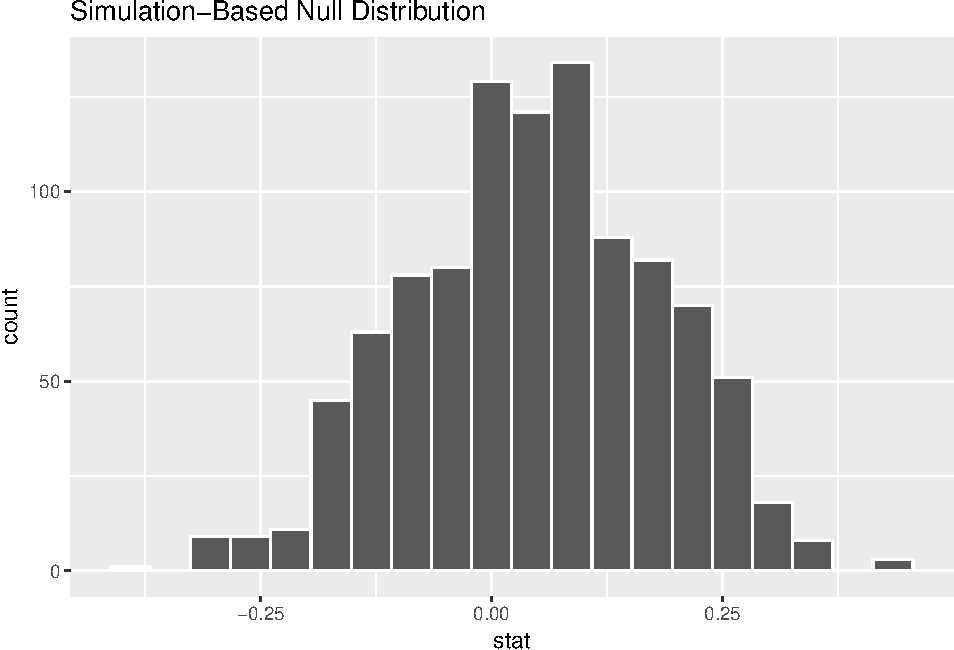
\includegraphics{DAWeek7_files/figure-latex/yawn_generate-1.pdf}

This distribution is roughly symmetric and bell-shaped but isn't quite
there. Let's use the percentile-based method to compute a 95\%
confidence interval for the true difference in the proportion of those
that yawn with and without a seed presented. The arguments are
explicitly listed here but remember they are the defaults and simply
\texttt{get\_ci()} can be used.

\begin{Shaded}
\begin{Highlighting}[]
\NormalTok{bootstrap_distribution }\OperatorTok\StringTok{ }
\StringTok{  }\KeywordTok{get_ci}\NormalTok{(}\DataTypeTok{type =} \StringTok{"percentile"}\NormalTok{, }\DataTypeTok{level =} \FloatTok{0.95}\NormalTok{)}
\end{Highlighting}
\end{Shaded}

\begin{verbatim}
# A tibble: 1 x 2
  `2.5%` `97.5%`
   <dbl>   <dbl>
1 -0.219   0.293
\end{verbatim}

\emph{The confidence interval shown here is (-0.22, 0.29) and thus
includes the value of 0. Therefore zero is a plausible value for the
difference in the proportion of people that yawned with and without
seeing someone yawn which is inconclusive evidence of a relationship
between seeing someone yawn and yawning}

Therefore, we are not sure which proportion is larger. Some of the
bootstrap statistics showed the proportion without a seed to be higher
and others showed the proportion with a seed to be higher. If the
confidence interval was entirely above zero, we would be relatively sure
(about ``95\% confident'') that the seed group had a higher proportion
of yawning than the control group.

Note that this all relates to the importance of denoting the
\texttt{order} argument in the \texttt{calculate()} function. Since we
specified \texttt{"seed"} and then \texttt{"control"} positive values
for the statistic correspond to the \texttt{"seed"} proportion being
higher, whereas negative values correspond to the \texttt{"control"}
group being higher.

We, therefore, have evidence via this confidence interval suggesting
that the conclusion from the Mythbusters show that ``yawning is
contagious'' being ``confirmed'' is \textbf{not} statistically correct.

\section{Further Tasks}\label{further-tasks}

\subsection{Confidence Intervals for Yawn
Data}\label{confidence-intervals-for-yawn-data}

In the last section, we constructed a confidence interval for the
difference in the proportion of people who yawned between the ``seeded''
group and the ``control'' group (Scenario 3).

By modifying the code in the last section in light of how we constructed
a confidence interval for the age of pennies in the section on
``Constructing confidence intervals'' (Scenario 2), use
mythbusters\_yawn data to constuct a confidence interval for the
proportion of people who yawn when they see someone else yawn (Scenario
1). Does this overlap with the confidence interval for the proportion of
people who yawn when they did not see someone else yawn (Scenario 1
again!)? Are your findings here consistent with the findings in the last
section?

\begin{Shaded}
\begin{Highlighting}[]
\NormalTok{bootstrap_distribution <-}\StringTok{ }\NormalTok{mythbusters_yawn }\OperatorTok
\StringTok{  }\KeywordTok{filter}\NormalTok{(group}\OperatorTok{==}\StringTok{"seed"}\NormalTok{) }\OperatorTok
\StringTok{  }\KeywordTok{specify}\NormalTok{(}\DataTypeTok{formula =}\NormalTok{ yawn }\OperatorTok{~}\StringTok{ }\OtherTok{NULL}\NormalTok{, }\DataTypeTok{success =} \StringTok{"yes"}\NormalTok{) }\OperatorTok
\StringTok{  }\KeywordTok{generate}\NormalTok{(}\DataTypeTok{reps =} \DecValTok{1000}\NormalTok{) }\OperatorTok
\StringTok{  }\KeywordTok{calculate}\NormalTok{(}\DataTypeTok{stat =} \StringTok{"prop"}\NormalTok{)}
\NormalTok{bootstrap_distribution }\OperatorTok\StringTok{ }\KeywordTok{visualize}\NormalTok{(}\DataTypeTok{bins =} \DecValTok{20}\NormalTok{)}
\end{Highlighting}
\end{Shaded}

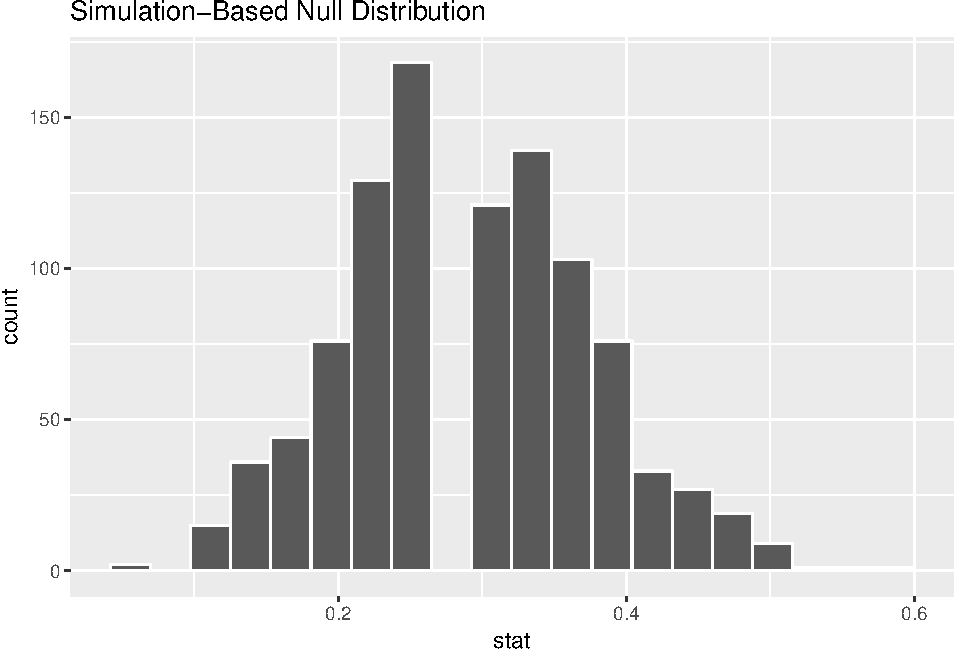
\includegraphics{DAWeek7_files/figure-latex/yawn_get_ci2-1.pdf}

This distribution is roughly symmetric and bell-shaped but isn't quite
there. Let's use the percentile-based method to compute a 95\%
confidence interval for the true proportion of those that yawn with a
seed presented. The arguments are explicitly listed here but remember
they are the defaults and simply get\_ci() can be used.

\begin{Shaded}
\begin{Highlighting}[]
\NormalTok{bootstrap_distribution }\OperatorTok
\StringTok{  }\KeywordTok{get_ci}\NormalTok{(}\DataTypeTok{type =} \StringTok{"percentile"}\NormalTok{, }\DataTypeTok{level =} \FloatTok{0.95}\NormalTok{)}
\end{Highlighting}
\end{Shaded}

\begin{verbatim}
# A tibble: 1 x 2
  `2.5%` `97.5%`
   <dbl>   <dbl>
1  0.147   0.471
\end{verbatim}

The confidence interval shown here is (0.15, 0.44). The range of
plausible values for the proportion of people that yawned with after
seeing someone yawn is therefore between 0.15 and 0.44. We now repeat
the exercise but for the group that didn't see someone yawn, i.e.
\texttt{group\ ==\ "control"}

\begin{Shaded}
\begin{Highlighting}[]
\NormalTok{bootstrap_distribution <-}\StringTok{ }\NormalTok{mythbusters_yawn }\OperatorTok
\StringTok{  }\KeywordTok{filter}\NormalTok{(group}\OperatorTok{==}\StringTok{"control"}\NormalTok{) }\OperatorTok
\StringTok{  }\KeywordTok{specify}\NormalTok{(}\DataTypeTok{formula =}\NormalTok{ yawn }\OperatorTok{~}\StringTok{ }\OtherTok{NULL}\NormalTok{, }\DataTypeTok{success =} \StringTok{"yes"}\NormalTok{) }\OperatorTok
\StringTok{  }\KeywordTok{generate}\NormalTok{(}\DataTypeTok{reps =} \DecValTok{1000}\NormalTok{) }\OperatorTok
\StringTok{  }\KeywordTok{calculate}\NormalTok{(}\DataTypeTok{stat =} \StringTok{"prop"}\NormalTok{)}
\NormalTok{bootstrap_distribution }\OperatorTok\StringTok{ }\KeywordTok{visualize}\NormalTok{(}\DataTypeTok{bins =} \DecValTok{20}\NormalTok{)}
\end{Highlighting}
\end{Shaded}

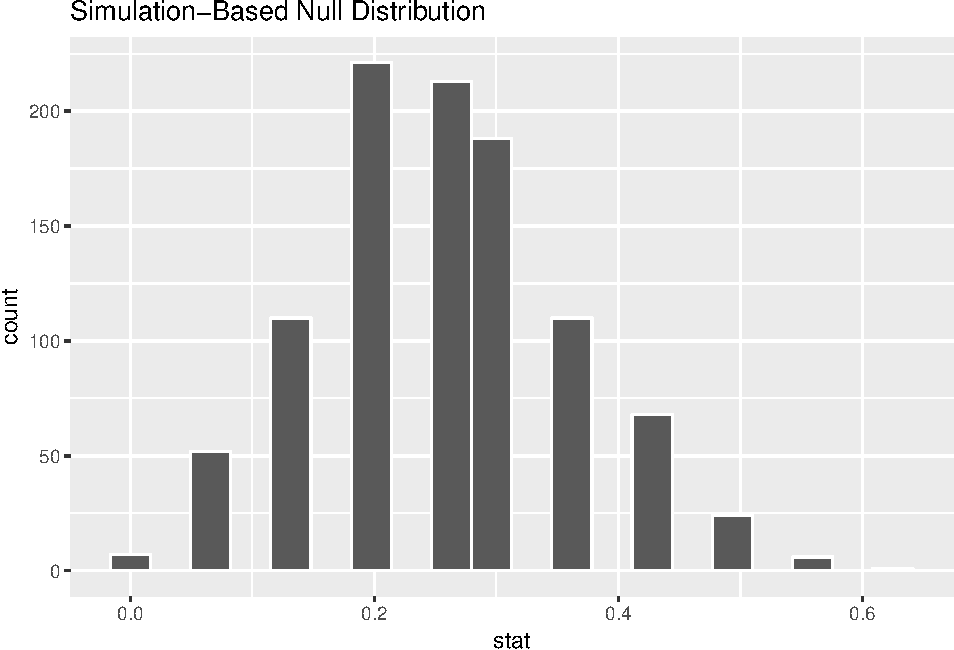
\includegraphics{DAWeek7_files/figure-latex/yawn_get_ci4-1.pdf}

\begin{Shaded}
\begin{Highlighting}[]
\NormalTok{bootstrap_distribution }\OperatorTok
\StringTok{  }\KeywordTok{get_ci}\NormalTok{(}\DataTypeTok{type =} \StringTok{"percentile"}\NormalTok{, }\DataTypeTok{level =} \FloatTok{0.95}\NormalTok{)}
\end{Highlighting}
\end{Shaded}

\begin{verbatim}
# A tibble: 1 x 2
  `2.5%` `97.5%`
   <dbl>   <dbl>
1 0.0625     0.5
\end{verbatim}

Setting \texttt{type\ =\ "bootstrap"} in \texttt{generate()}. The
confidence interval shown here is (0.06, 0.5). The range of plausible
values for the proportion of people that yawned without seeing someone
yawn is therefore between 0.06 and 0.5.

Comparing the two CIs for the proportion of those that saw someone yawn
(0.15, 0.44) and those that didn't (0.06, 0.5), we note that these two
CIs overlap, which is consistent with the findings from the CI for the
difference in the two proptions (-0.23, 0.31) in the last section,
i.e.~since they \textbf{do overlap} its plausible that they could each
take the \emph{same value} and therefore its plausible that their
\textbf{difference is zero}, which is exactly what the CI for the
difference in proportions tells us.

\subsection{Confidence Interval for Cats
Data}\label{confidence-interval-for-cats-data}

Recall the data on 144 domestic male and female adult cats that we first
saw in Week 4. Each cat had their heart weight in grams (Hwt) and body
weight in kilograms (Bwt) measured, and interest lies in exploring
difference between females and males. a. Construct a bootstrap
confidence intervals for the avearge heart weight of female and male
cats separately? Interpret your results. b. Construct a bootstrap
confidence interval for the difference in the avearge heart weights of
female and male cats. Interpret your result. c. Repeat a. and b. for the
body weight of cats. Hint: You need to read in the cats data and remind
yourself how it is organised, e.g.

\begin{Shaded}
\begin{Highlighting}[]
\NormalTok{cats <-}\StringTok{ }\KeywordTok{read.csv}\NormalTok{(}\StringTok{"cats.csv"}\NormalTok{)}
\KeywordTok{glimpse}\NormalTok{(cats)}
\end{Highlighting}
\end{Shaded}

\begin{verbatim}
Observations: 144
Variables: 4
$ X   <int> 1, 2, 3, 4, 5, 6, 7, 8, 9, 10, 11, 12, 13, 14, 15, 16, 17,...
$ Sex <fct> F, F, F, F, F, F, F, F, F, F, F, F, F, F, F, F, F, F, F, F...
$ Bwt <dbl> 2.0, 2.0, 2.0, 2.1, 2.1, 2.1, 2.1, 2.1, 2.1, 2.1, 2.1, 2.1...
$ Hwt <dbl> 7.0, 7.4, 9.5, 7.2, 7.3, 7.6, 8.1, 8.2, 8.3, 8.5, 8.7, 9.8...
\end{verbatim}

\textbf{Solution 2.a.}

\begin{enumerate}
\def\labelenumi{\alph{enumi}.}
\tightlist
\item
  Construct a bootstrap confidence intervals for the avearge heart
  weight of female and male cats separately? Interpret your results.
\end{enumerate}

We start by focusing on female cats, i.e.~Sex == ``F'':

\begin{Shaded}
\begin{Highlighting}[]
\NormalTok{cats <-}\StringTok{ }\KeywordTok{read.csv}\NormalTok{(}\StringTok{"cats.csv"}\NormalTok{)}
\CommentTok{#glimpse(cats)}
\NormalTok{bootstrap_distribution <-}\StringTok{ }\NormalTok{cats }\OperatorTok
\StringTok{  }\KeywordTok{filter}\NormalTok{(Sex }\OperatorTok{==}\StringTok{ "F"}\NormalTok{) }\OperatorTok
\StringTok{  }\KeywordTok{specify}\NormalTok{(}\DataTypeTok{response =}\NormalTok{ Hwt) }\OperatorTok
\StringTok{  }\KeywordTok{generate}\NormalTok{(}\DataTypeTok{reps =} \DecValTok{1000}\NormalTok{) }\OperatorTok
\StringTok{  }\KeywordTok{calculate}\NormalTok{(}\DataTypeTok{stat =} \StringTok{"mean"}\NormalTok{)}

\CommentTok{#bootstrap_distribution %>% visualize()}
 
\NormalTok{percentile_ci <-}\StringTok{ }\NormalTok{bootstrap_distribution }\OperatorTok
\StringTok{  }\KeywordTok{get_ci}\NormalTok{()}
\CommentTok{#percentile_ci}
\end{Highlighting}
\end{Shaded}

Using the percentile method, our range of plausible values for the mean
heart weight of female adult cats is 8.82 grams to 9.58 grams.

Now repeat the analysis for male cats, i.e.~Sex == ``M'':

\begin{Shaded}
\begin{Highlighting}[]
\NormalTok{bootstrap_distribution <-}\StringTok{ }\NormalTok{cats }\OperatorTok
\StringTok{  }\KeywordTok{filter}\NormalTok{(Sex }\OperatorTok{==}\StringTok{ "M"}\NormalTok{) }\OperatorTok
\StringTok{  }\KeywordTok{specify}\NormalTok{(}\DataTypeTok{response =}\NormalTok{ Hwt) }\OperatorTok
\StringTok{  }\KeywordTok{generate}\NormalTok{(}\DataTypeTok{reps =} \DecValTok{1000}\NormalTok{) }\OperatorTok
\StringTok{  }\KeywordTok{calculate}\NormalTok{(}\DataTypeTok{stat =} \StringTok{"mean"}\NormalTok{)}

\CommentTok{#bootstrap_distribution %>% visualize()}
\NormalTok{percentile_ci <-}\StringTok{ }\NormalTok{bootstrap_distribution }\OperatorTok
\StringTok{  }\KeywordTok{get_ci}\NormalTok{()}
\CommentTok{#percentile_ci}
\end{Highlighting}
\end{Shaded}

Using the percentile method, our range of plausible values for the mean
heart weight of male adult cats is 10.83 grams to 11.79 grams.

\textbf{Solution 2.b.}

\begin{enumerate}
\def\labelenumi{\alph{enumi}.}
\setcounter{enumi}{1}
\tightlist
\item
  Construct a bootstrap confidence interval for the difference in the
  avearge heart weights of female and male cats. Interpret your result.
\end{enumerate}

\begin{Shaded}
\begin{Highlighting}[]
\NormalTok{bootstrap_distribution <-}\StringTok{ }\NormalTok{cats }\OperatorTok
\StringTok{  }\KeywordTok{specify}\NormalTok{(Hwt}\OperatorTok{~}\NormalTok{Sex) }\OperatorTok
\StringTok{  }\KeywordTok{generate}\NormalTok{(}\DataTypeTok{reps =} \DecValTok{1000}\NormalTok{) }\OperatorTok
\StringTok{  }\KeywordTok{calculate}\NormalTok{(}\DataTypeTok{stat =} \StringTok{"diff in means"}\NormalTok{, }\DataTypeTok{order =} \KeywordTok{c}\NormalTok{(}\StringTok{"F"}\NormalTok{, }\StringTok{"M"}\NormalTok{))}
\NormalTok{  percentile_ci <-}\StringTok{ }\NormalTok{bootstrap_distribution }\OperatorTok
\StringTok{  }\KeywordTok{get_ci}\NormalTok{()}
\end{Highlighting}
\end{Shaded}

Using the percentile method, our range of plausible values for the
difference in the mean heart weight between female and male adult cats
is -2.77 grams to -1.45 grams. That is to say that on average female
adult cats' hearts weigh between 1.45 and 2.77 grams less than adult
male cats' hearts. (Note: the fact that the individual CIs in part a.
didn't overlap told us that zero wouldn't be in the interval for the
difference in the population means)

\textbf{Solution 2.c.}

\begin{enumerate}
\def\labelenumi{\alph{enumi}.}
\setcounter{enumi}{2}
\tightlist
\item
  Repeat a. and b. for the body weight of cats.
\end{enumerate}

RMarkdown makes it very easy to repeat the analysis in parts a. and b.
on a different variable.

\begin{Shaded}
\begin{Highlighting}[]
\NormalTok{cats <-}\StringTok{ }\KeywordTok{read.csv}\NormalTok{(}\StringTok{"cats.csv"}\NormalTok{)}
\NormalTok{bootstrap_distribution <-}\StringTok{ }\NormalTok{cats }\OperatorTok
\StringTok{  }\KeywordTok{filter}\NormalTok{(Sex }\OperatorTok{==}\StringTok{ "F"}\NormalTok{) }\OperatorTok
\StringTok{  }\KeywordTok{specify}\NormalTok{(}\DataTypeTok{response =}\NormalTok{ Bwt) }\OperatorTok
\StringTok{  }\KeywordTok{generate}\NormalTok{(}\DataTypeTok{reps =} \DecValTok{1000}\NormalTok{) }\OperatorTok
\StringTok{  }\KeywordTok{calculate}\NormalTok{(}\DataTypeTok{stat =} \StringTok{"mean"}\NormalTok{)}
\NormalTok{percentile_ci <-}\StringTok{ }\NormalTok{bootstrap_distribution }\OperatorTok
\StringTok{  }\KeywordTok{get_ci}\NormalTok{()}
\end{Highlighting}
\end{Shaded}

Using the percentile method, our range of plausible values for the mean
body weight of female adult cats is 2.28 kilograms to 2.43 kilograms.

Now repeat the analysis for male cats, i.e.~Sex == ``M'':

\begin{Shaded}
\begin{Highlighting}[]
\NormalTok{bootstrap_distribution <-}\StringTok{ }\NormalTok{cats }\OperatorTok
\StringTok{  }\KeywordTok{filter}\NormalTok{(Sex }\OperatorTok{==}\StringTok{ "M"}\NormalTok{) }\OperatorTok
\StringTok{  }\KeywordTok{specify}\NormalTok{(}\DataTypeTok{response =}\NormalTok{ Bwt) }\OperatorTok
\StringTok{  }\KeywordTok{generate}\NormalTok{(}\DataTypeTok{reps =} \DecValTok{1000}\NormalTok{) }\OperatorTok
\StringTok{  }\KeywordTok{calculate}\NormalTok{(}\DataTypeTok{stat =} \StringTok{"mean"}\NormalTok{)}
\NormalTok{percentile_ci <-}\StringTok{ }\NormalTok{bootstrap_distribution }\OperatorTok
\StringTok{  }\KeywordTok{get_ci}\NormalTok{()}
\end{Highlighting}
\end{Shaded}

Using the percentile method, our range of plausible values for the mean
body weight of male adult cats is 2.82 kilograms to 2.99 kilograms.

\begin{Shaded}
\begin{Highlighting}[]
\NormalTok{bootstrap_distribution <-}\StringTok{ }\NormalTok{cats }\OperatorTok
\StringTok{  }\KeywordTok{specify}\NormalTok{(Bwt}\OperatorTok{~}\NormalTok{Sex) }\OperatorTok
\StringTok{  }\KeywordTok{generate}\NormalTok{(}\DataTypeTok{reps =} \DecValTok{1000}\NormalTok{) }\OperatorTok
\StringTok{  }\KeywordTok{calculate}\NormalTok{(}\DataTypeTok{stat =} \StringTok{"diff in means"}\NormalTok{, }\DataTypeTok{order =} \KeywordTok{c}\NormalTok{(}\StringTok{"F"}\NormalTok{, }\StringTok{"M"}\NormalTok{))}
\NormalTok{  percentile_ci <-}\StringTok{ }\NormalTok{bootstrap_distribution }\OperatorTok
\StringTok{  }\KeywordTok{get_ci}\NormalTok{()}
\end{Highlighting}
\end{Shaded}

Using the percentile method, our range of plausible values for the
difference in the mean body weight between female and male adult cats is
-0.67 kilograms to -0.41 kilograms. That is to say that on average
female adult cats' bodies weigh between 0.41 and 0.67 kilograms
\textbf{less} than adult male cats' bodies. (Note: the fact that the
individual CIs in part a. didn't overlap told us that zero wouldn't be
in the interval for the difference in the population means)


\end{document}
